\section{Case Study}\label{case-study}


To evaluate the effectiveness and performance of the theoretical frameworks proposed, simulations were conducted using a practical case study. The subsequent sections begin by introducing the network configuration. Then, the numerical optimization results are presented, followed by a generalization to the case of probabilistic line-of-sight (LoS) condition for ground user links.



\subsection{Network Setup}\label{experimental-setup}

\subsubsection{Deployment Setup}\label{Deployment-Setup}
We examine a practical cellular network that consists of $19$ sites arranged in a hexagonal layout, where the inter-site distance (ISD) is $500$ meters. The configuration of this network and the BS deployment site indices are depicted in Fig.~\ref{TWC-Normal-Size-UAV}. Each site, here denoted by $k$, is associated with three sectors or cells. These cells have BSs located at the same positions (denoted by vector $\bm{p}_{3\times k-2} = \bm{p}_{3\times k-1} = \bm{p}_{3\times k}$), but they have different azimuth orientations. Specifically, the azimuth orientations are $\phi_{3\times k-2} = 0^\circ, \phi_{3\times k-1} = 120^\circ\textrm{, and } \phi_{3\times k} = 240^\circ$. Hence, a total of $N=57$ BSs are present, each requiring optimization of its vertical antenna tilt and transmission power values. All BSs share a common height of $h_{n,\mathrm{B}} = 25$m for $n$ ranging from $1$ to $N=57$. The maximum transmission power allowed for all BSs is $43$\,dBm.


The ground users are spatially distributed across a square area  $Q_G = [-750, 750] \times [-750, 750]$ as shown in Fig. \ref{TWC-Normal-Size-GUE}. Their distribution follows a uniform density function $\lambda_\textrm{G}(\bm{q})$ and they are assumed to have a fixed height of $h_\textrm{G} = 1.5$\,m. The UAVs are distributed over four vertical aerial corridors, represented by $Q_U = Q_1\cup Q_2\cup Q_3 \cup Q_4$, following a uniform density function $\lambda_\textrm{U}(\bm{q})$. These corridors, illustrated in Fig. \ref{TWC-Normal-Size-UAV}, are defined as $Q_1 = [-770, -730]\times [-1000, 1000]$, $Q_2 = [-1000, 1000]\times [-770, -730]$, $Q_3 = [-1000, 1000]\times [730, 770]$, and $Q_4 = [730, 770]\times [-1000, 1000]$. The heights of the corridors are set to $h_1 = h_4 = 150$\,m and $h_2 = h_3 = 120$\,m. The overall density function $\lambda(\bm{q})$, which represents the user distribution in $Q = Q_G \cup Q_U$, is a mixture of $\lambda_\textrm{G}(\bm{q})$ and $\lambda_\textrm{U}(\bm{q})$. Specifically, $\lambda(\bm{q}) = r\lambda_\textrm{G}(\bm{q}) + (1-r) \lambda_\textrm{U}(\bm{q})$, where $r$ is the mixing ratio. Throughout the study, we consider three different values for the parameter $r$, namely $1$, $0$, and $0.5$. These values correspond to optimizing the cellular network exclusively for ground users, exclusively for UAVs, and for both ground users and UAVs with equal priority, respectively.



\subsubsection{Channel Setup}\label{Channel-Setup}

According to the specifications provided by 3GPP \cite{3GPP36777,3GPP38901}, for a carrier frequency of 2GHz and under line-of-sight conditions, the values of $a_{\bm{q}}$ and $b_{\bm{q}}$ are set as follows:
\begin{equation}\label{a_q_values}
a_{\bm{q}} =
\begin{cases}
34.02\,\textrm{dB}, & \text{if}\ \bm{q}\in Q_U, \\
38.42\,\textrm{dB}, & \text{if}\ \bm{q}\in Q_G,
\end{cases}
\end{equation}
\begin{equation}\label{b_q_values}
b_{\bm{q}} =
\begin{cases}
22 \textrm{ (for a pathloss exponent of 2.2)}, & \text{if}\ \bm{q}\in Q_U, \\
30 \textrm{ (for a pathloss exponent of 3.0)}, & \text{if}\ \bm{q}\in Q_G.
\end{cases}
\end{equation}

Furthermore, the directional antennas have the vertical half-power beamwidth of $\theta_\textrm{3dB} = 10^{\circ}$, the horizontal half-power beamwidth of $\phi_\textrm{3dB} = 65^{\circ}$, and the maximum antenna gain of $A_\textrm{max} = 14$\,dBi at the boresight.




\begin{figure*}[!t]
\centering
\subfloat[GUEs, setup as per Sec.~\ref{experimental-setup}.]{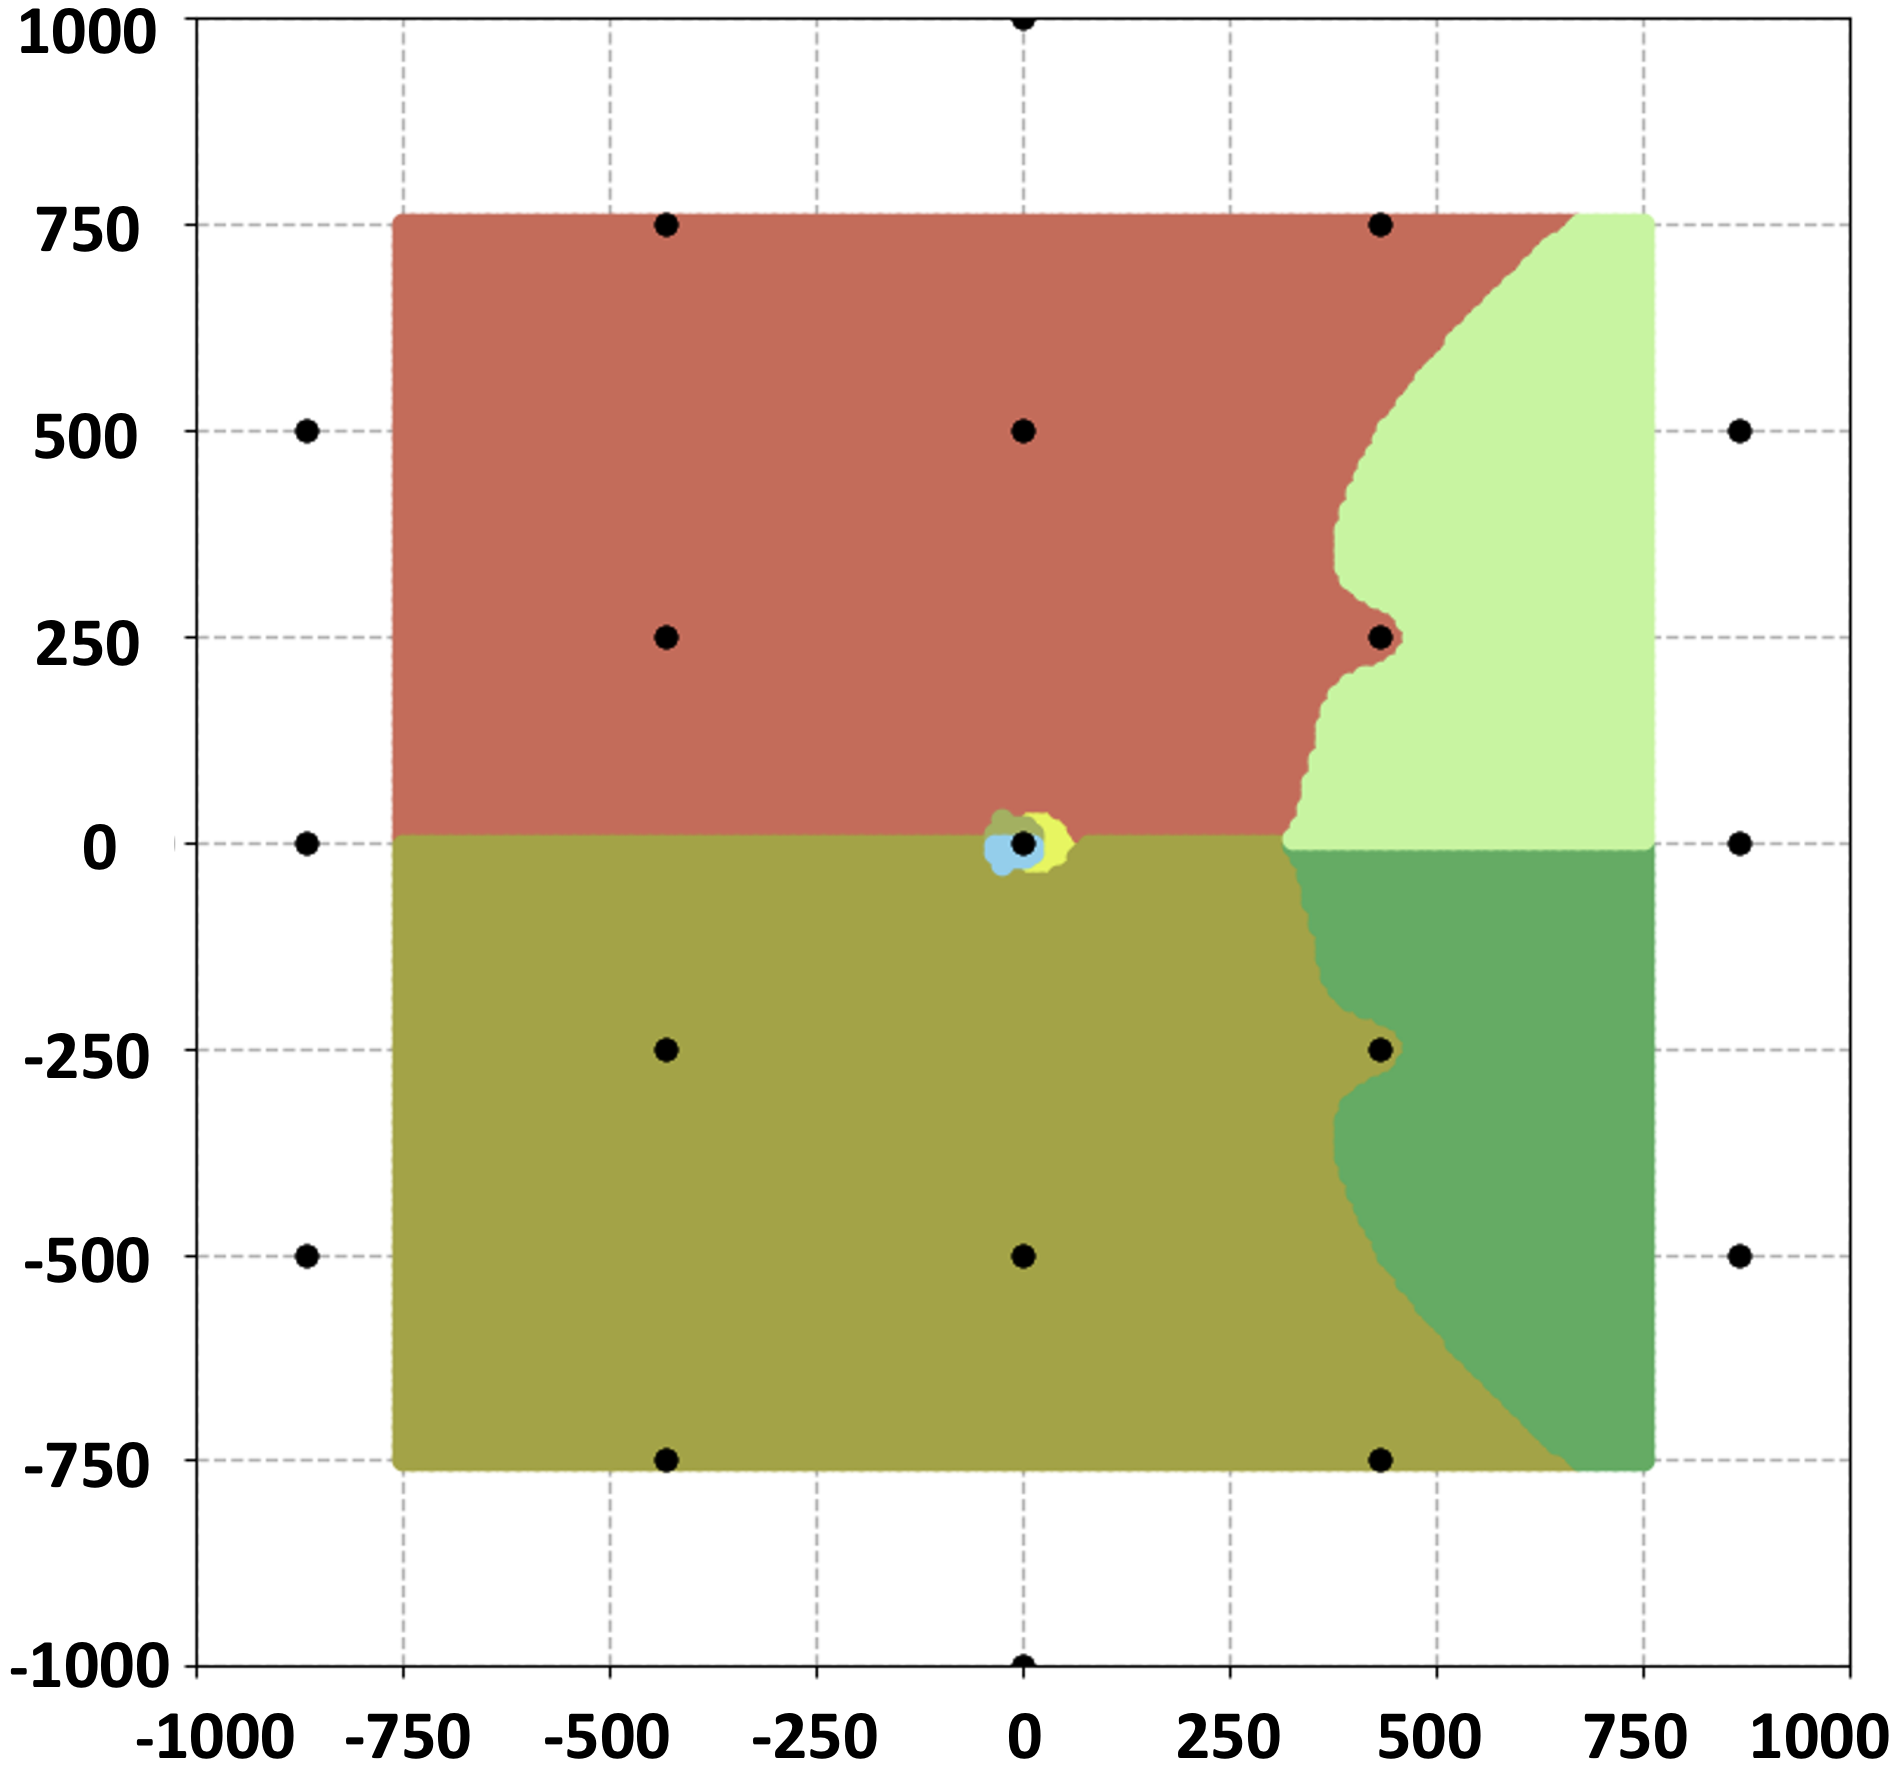
\includegraphics[width=56mm]{Figures/Exemplary-Cell-Partitioning/TWC-normal-size-SINR-GUE-Cells_1.png}
\label{TWC-Normal-Size-GUE}}
\hspace*{3mm}
\subfloat[GUEs, setup as per Section~\ref{experimental-setup} $\times$2.]{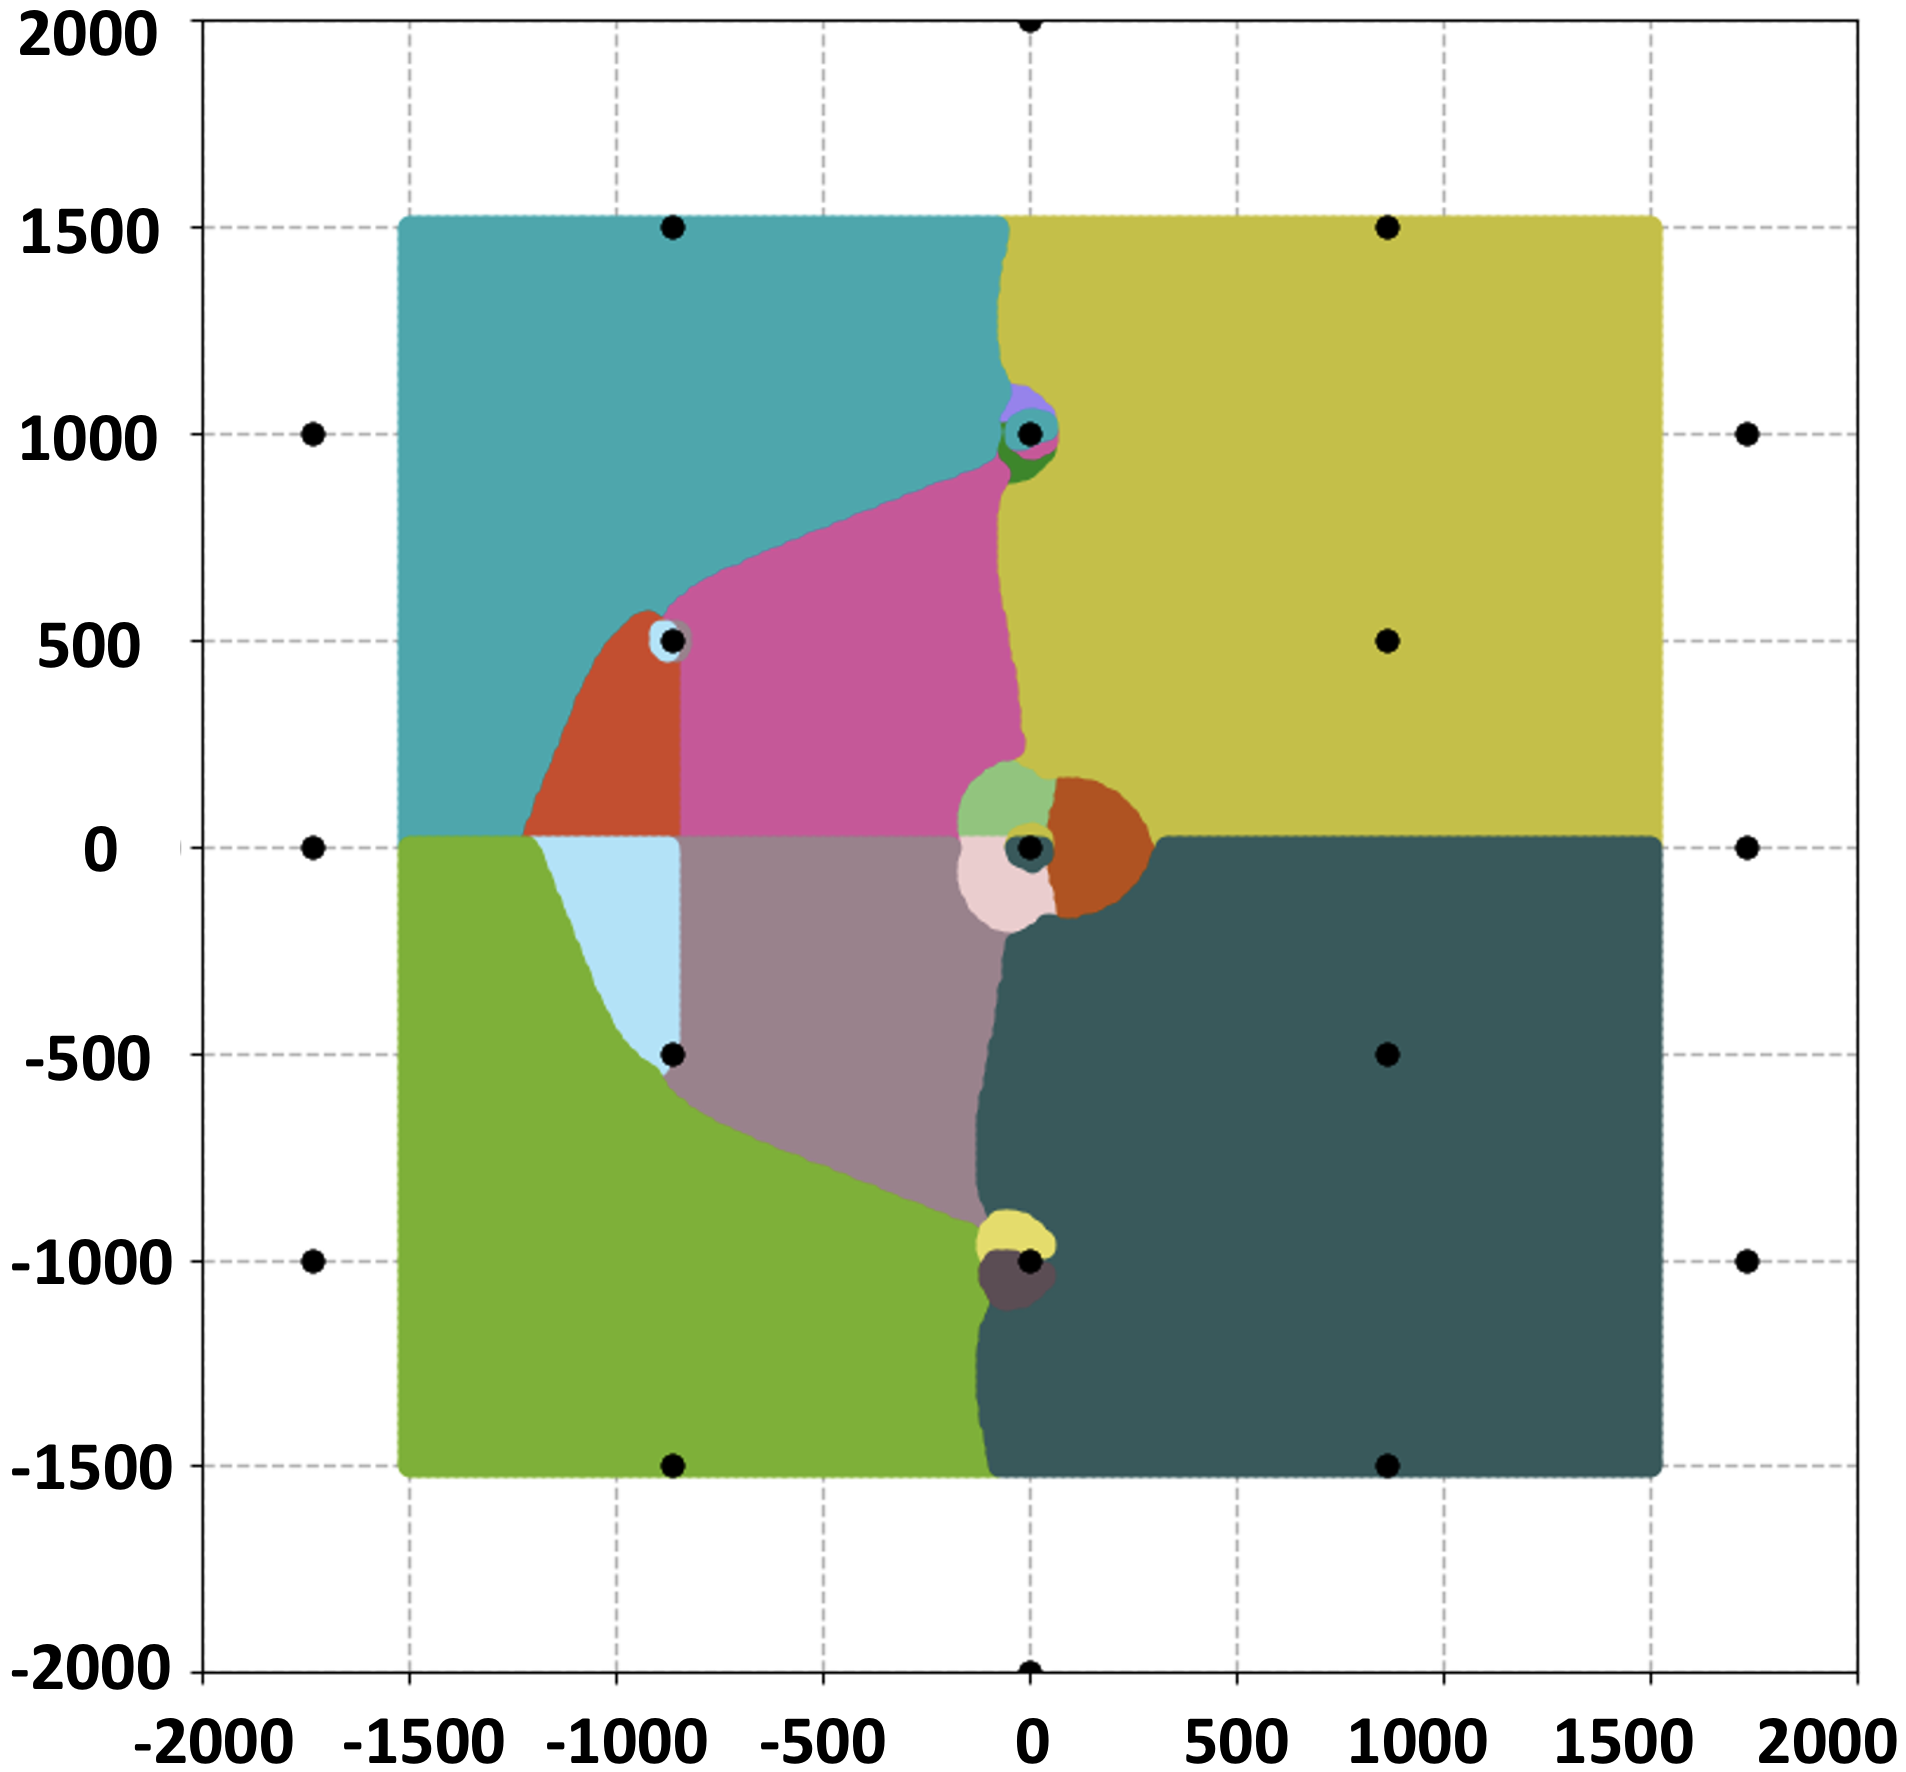
\includegraphics[width=56mm]{Figures/Exemplary-Cell-Partitioning/TWC-SINR-GUE-Large-Cells_4.png}
\label{TWC-Large-Size-GUE}}
\hspace*{3mm}
\subfloat[GUEs, setup as per Section~\ref{experimental-setup} $\times$4.]{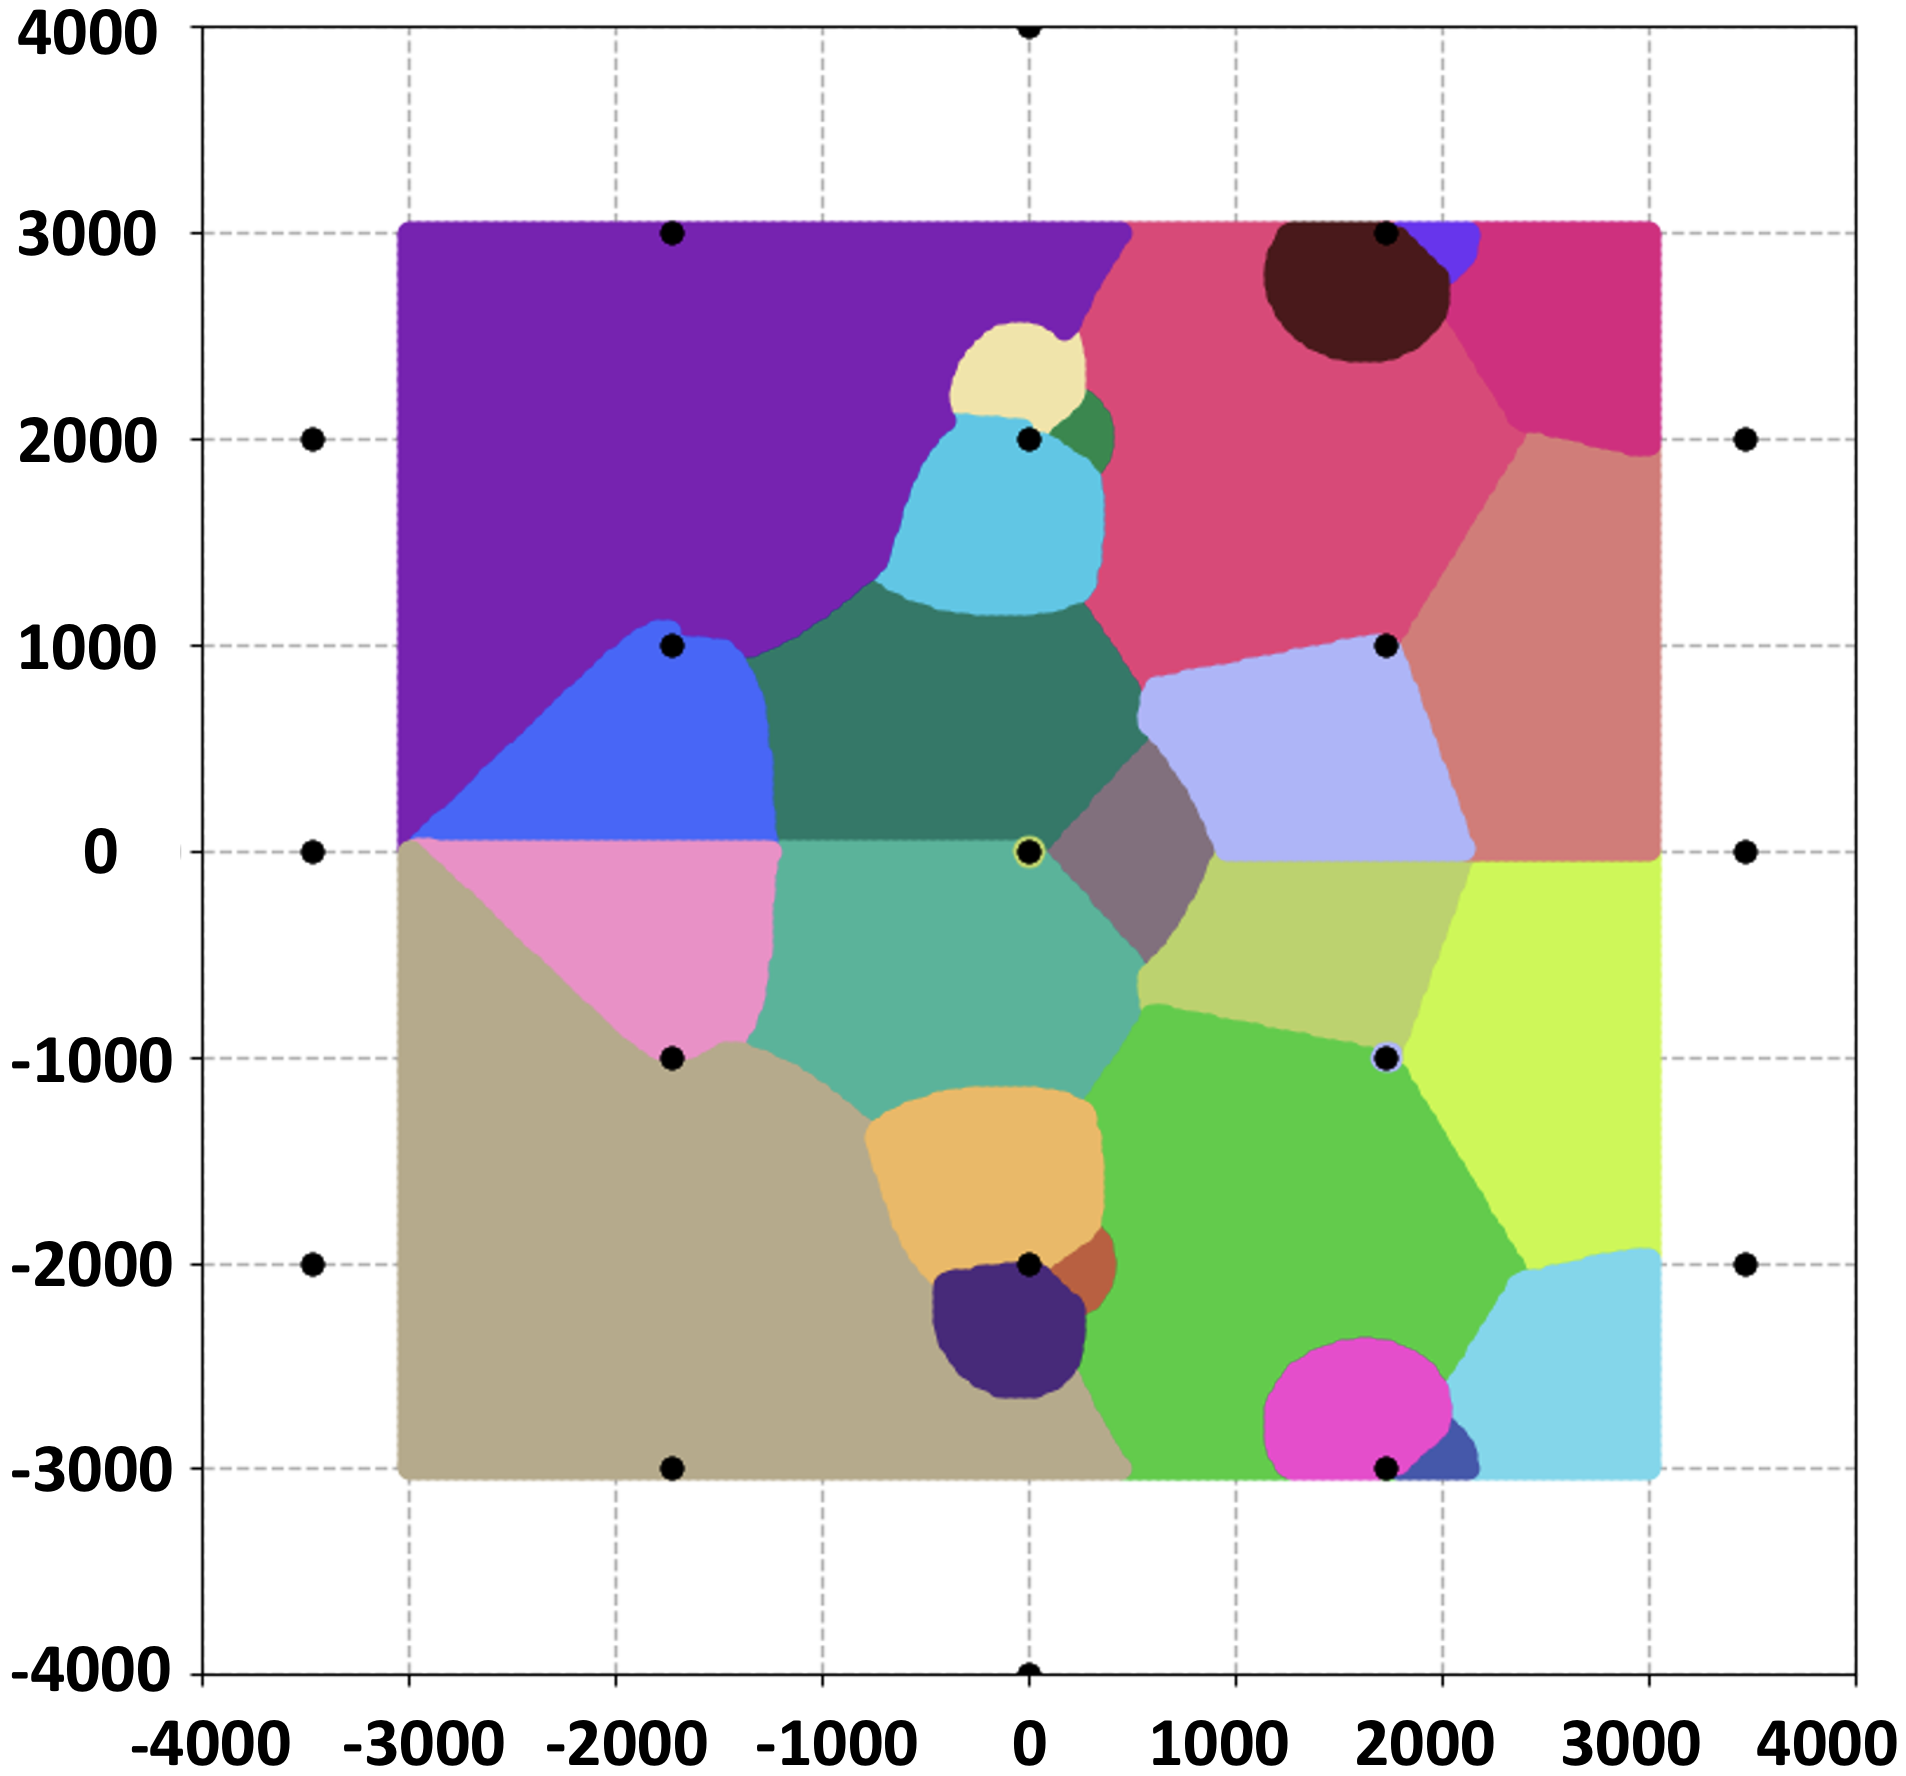
\includegraphics[width=56mm]{Figures/Exemplary-Cell-Partitioning/TWC-SINR-GUE-Very-Large-Cells_2.png}
\label{TWC-Very-Large-Size-GUE}}
\\\vspace*{3mm}
\subfloat[UAVs, setup as per Section~\ref{experimental-setup}.]{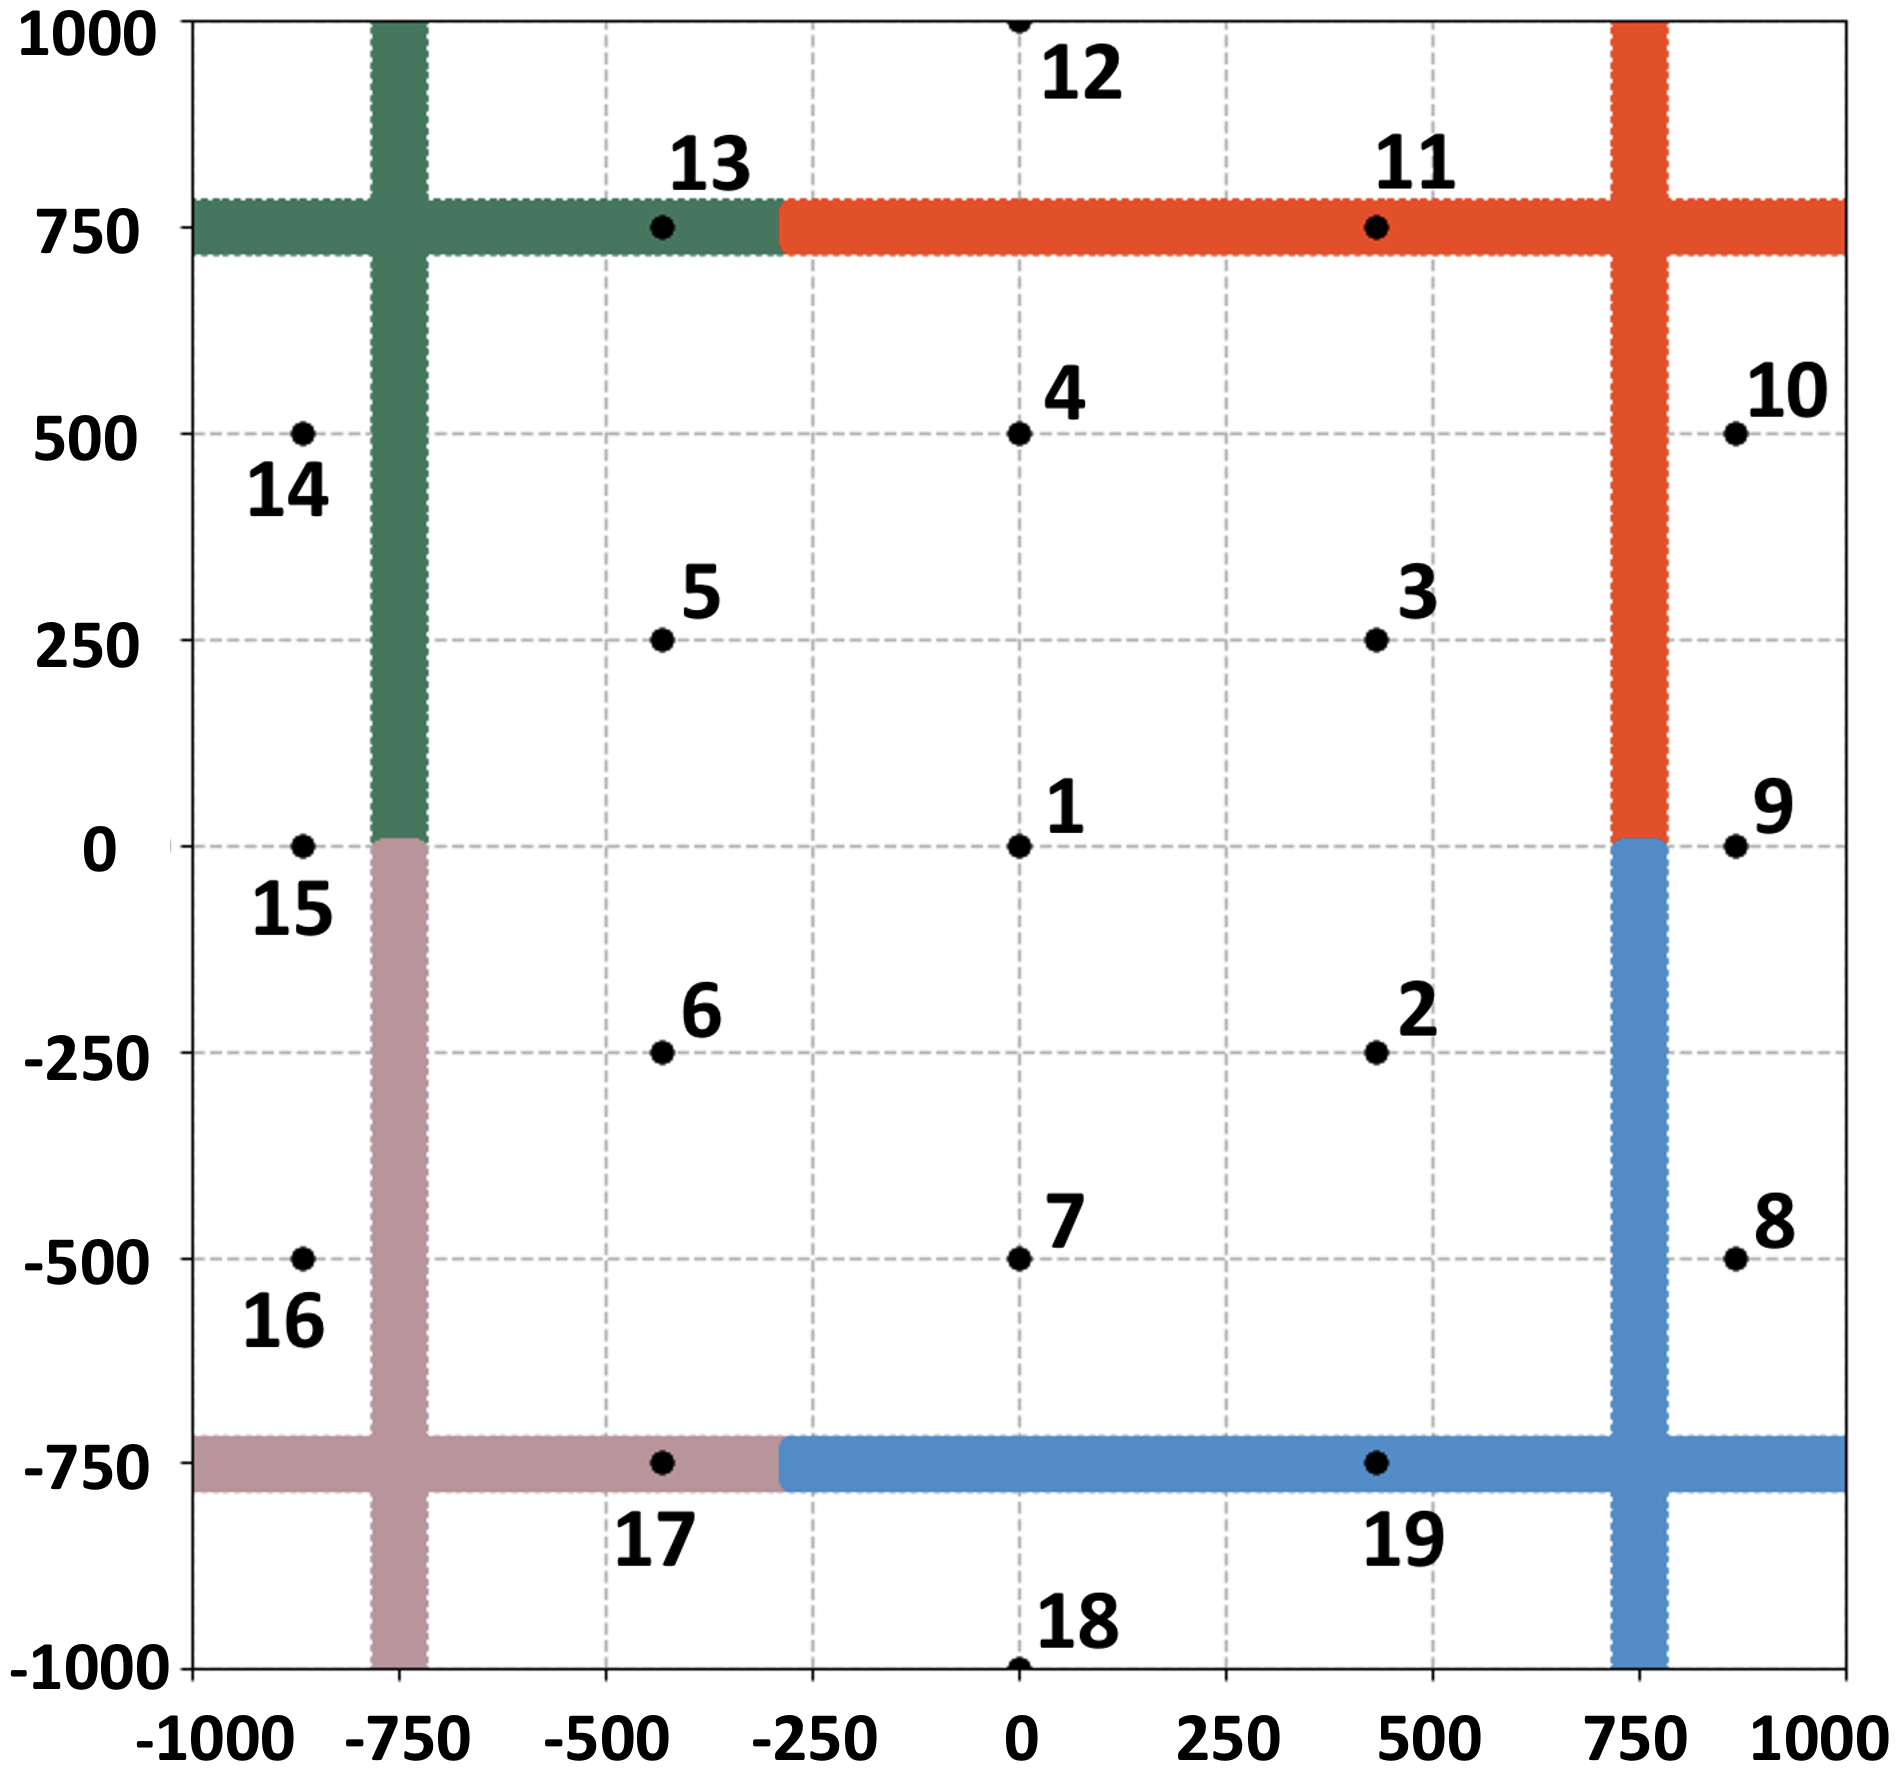
\includegraphics[width=56mm]{Figures/Exemplary-Cell-Partitioning/TWC-normal-size-UAV-target-region.png}
\label{TWC-Normal-Size-UAV}}
\hspace*{3mm}
\subfloat[UAVs, setup as per Section~\ref{experimental-setup} $\times$2.]{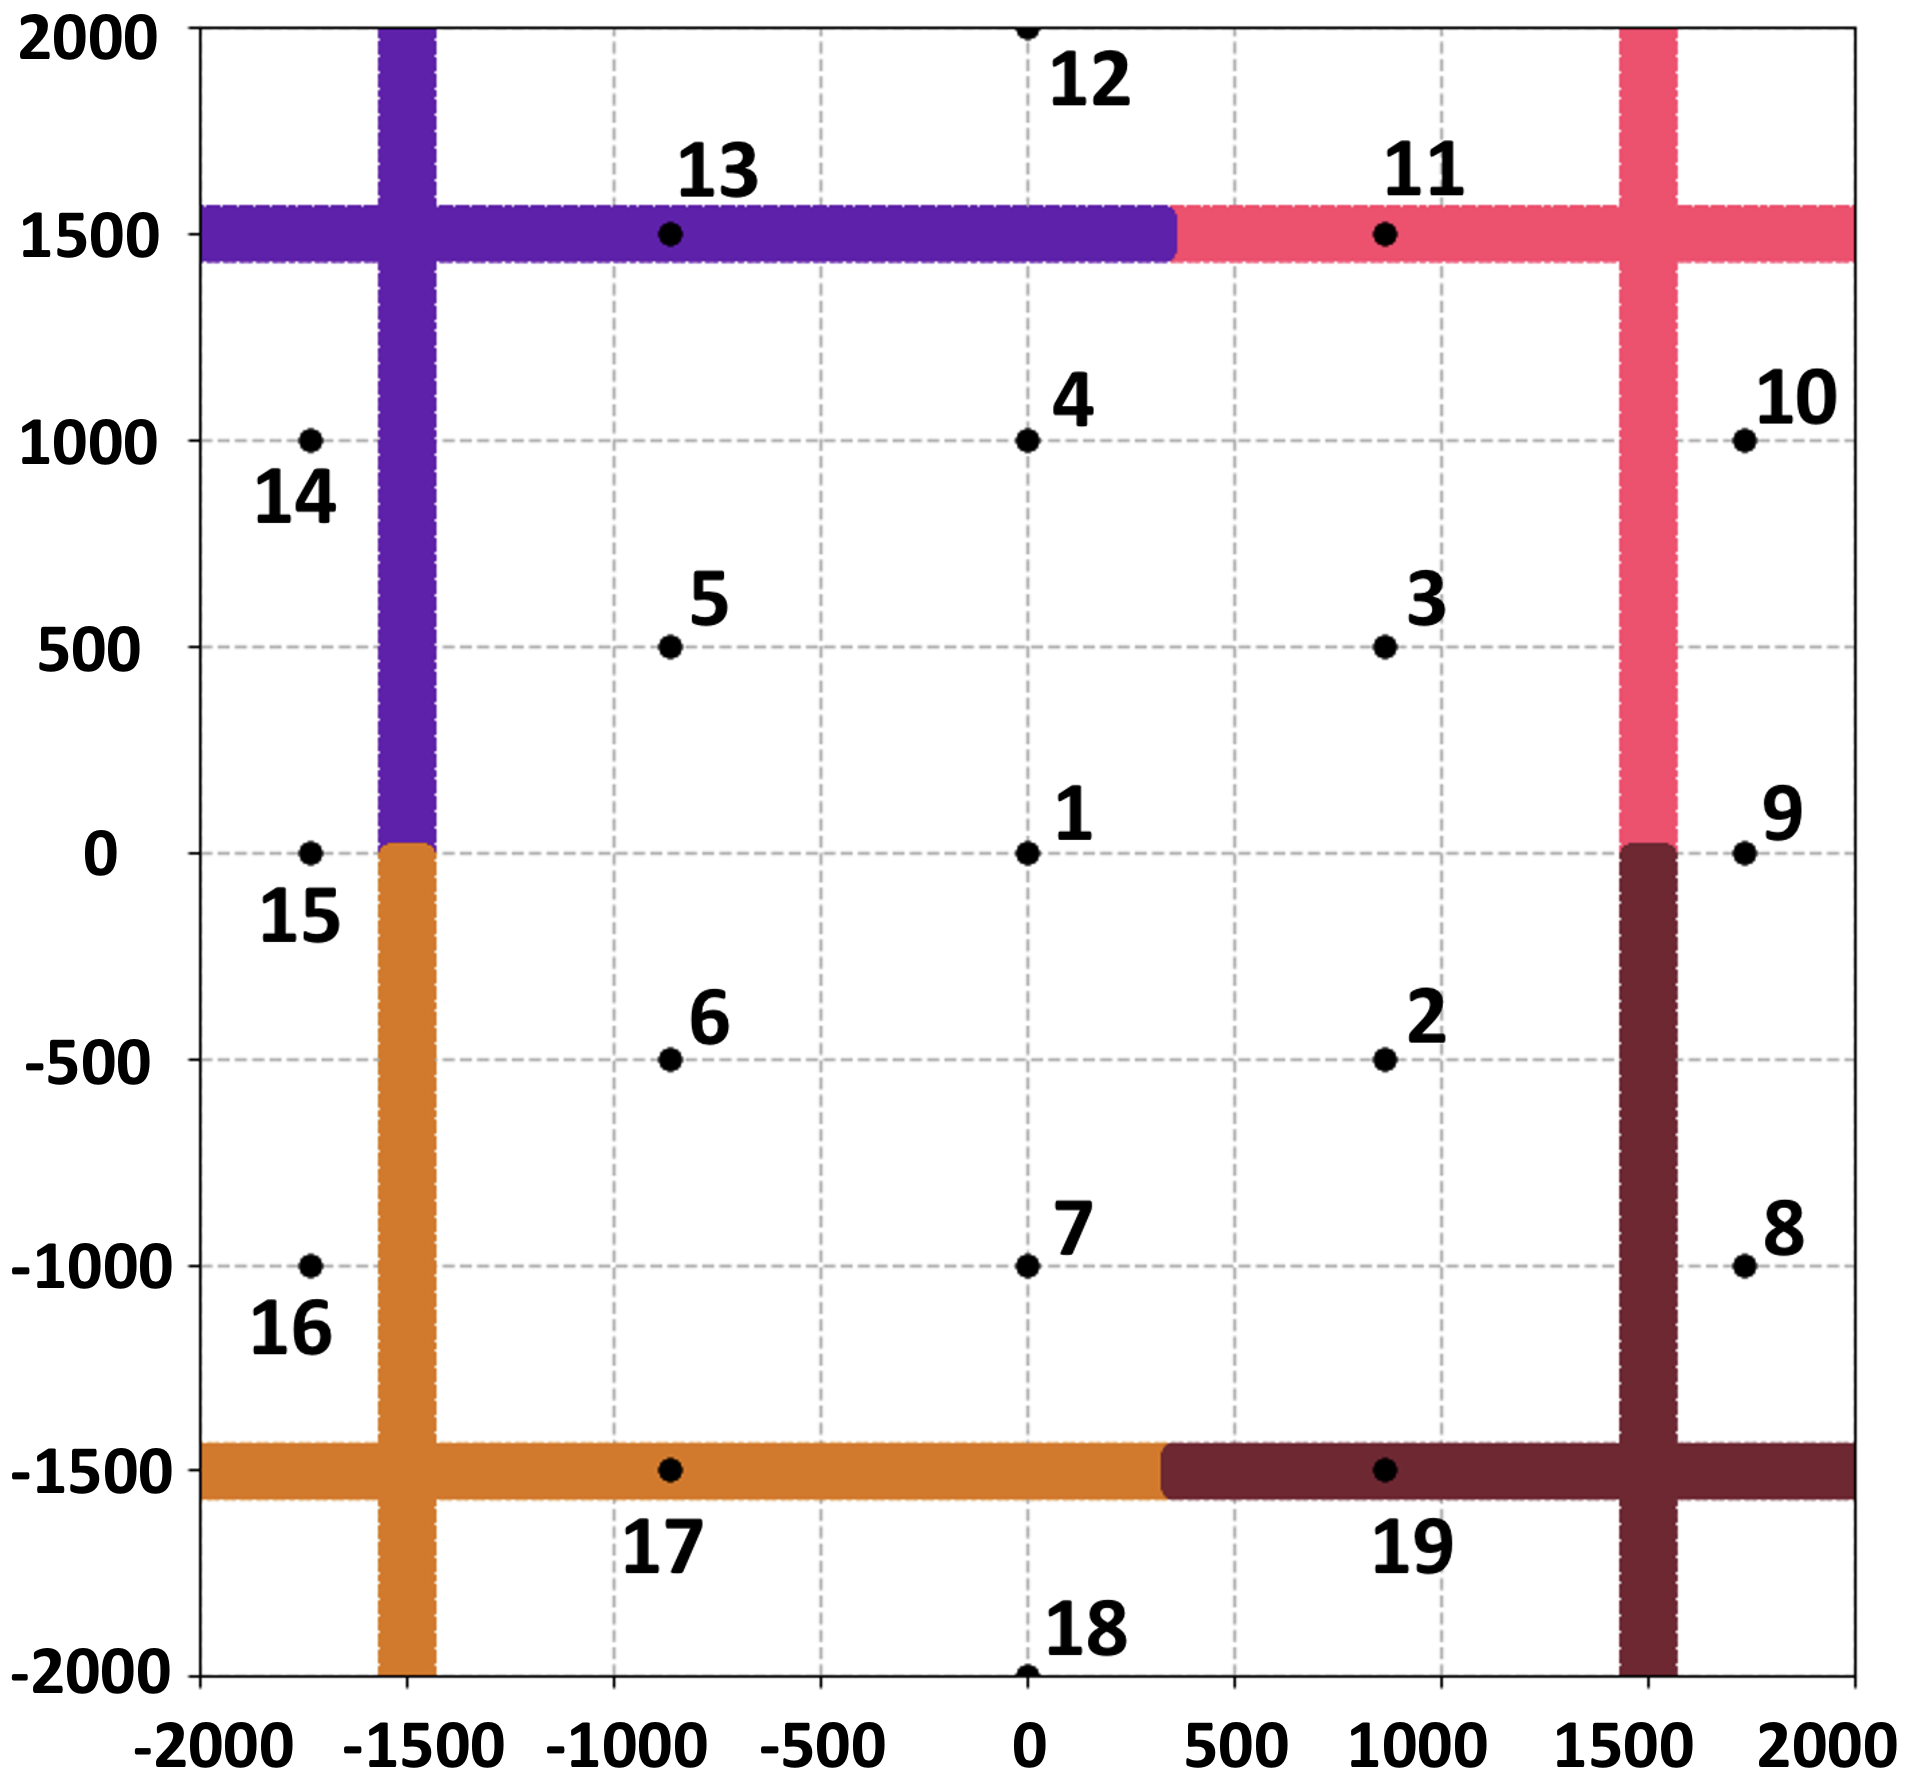
\includegraphics[width=56mm]{Figures/Exemplary-Cell-Partitioning/TWC-large-size-UAV-target-region-2.png}
\label{TWC-Large-Size-UAV}}
\hspace*{3mm}
\subfloat[UAVs, setup as per Section~\ref{experimental-setup} $\times$4.]{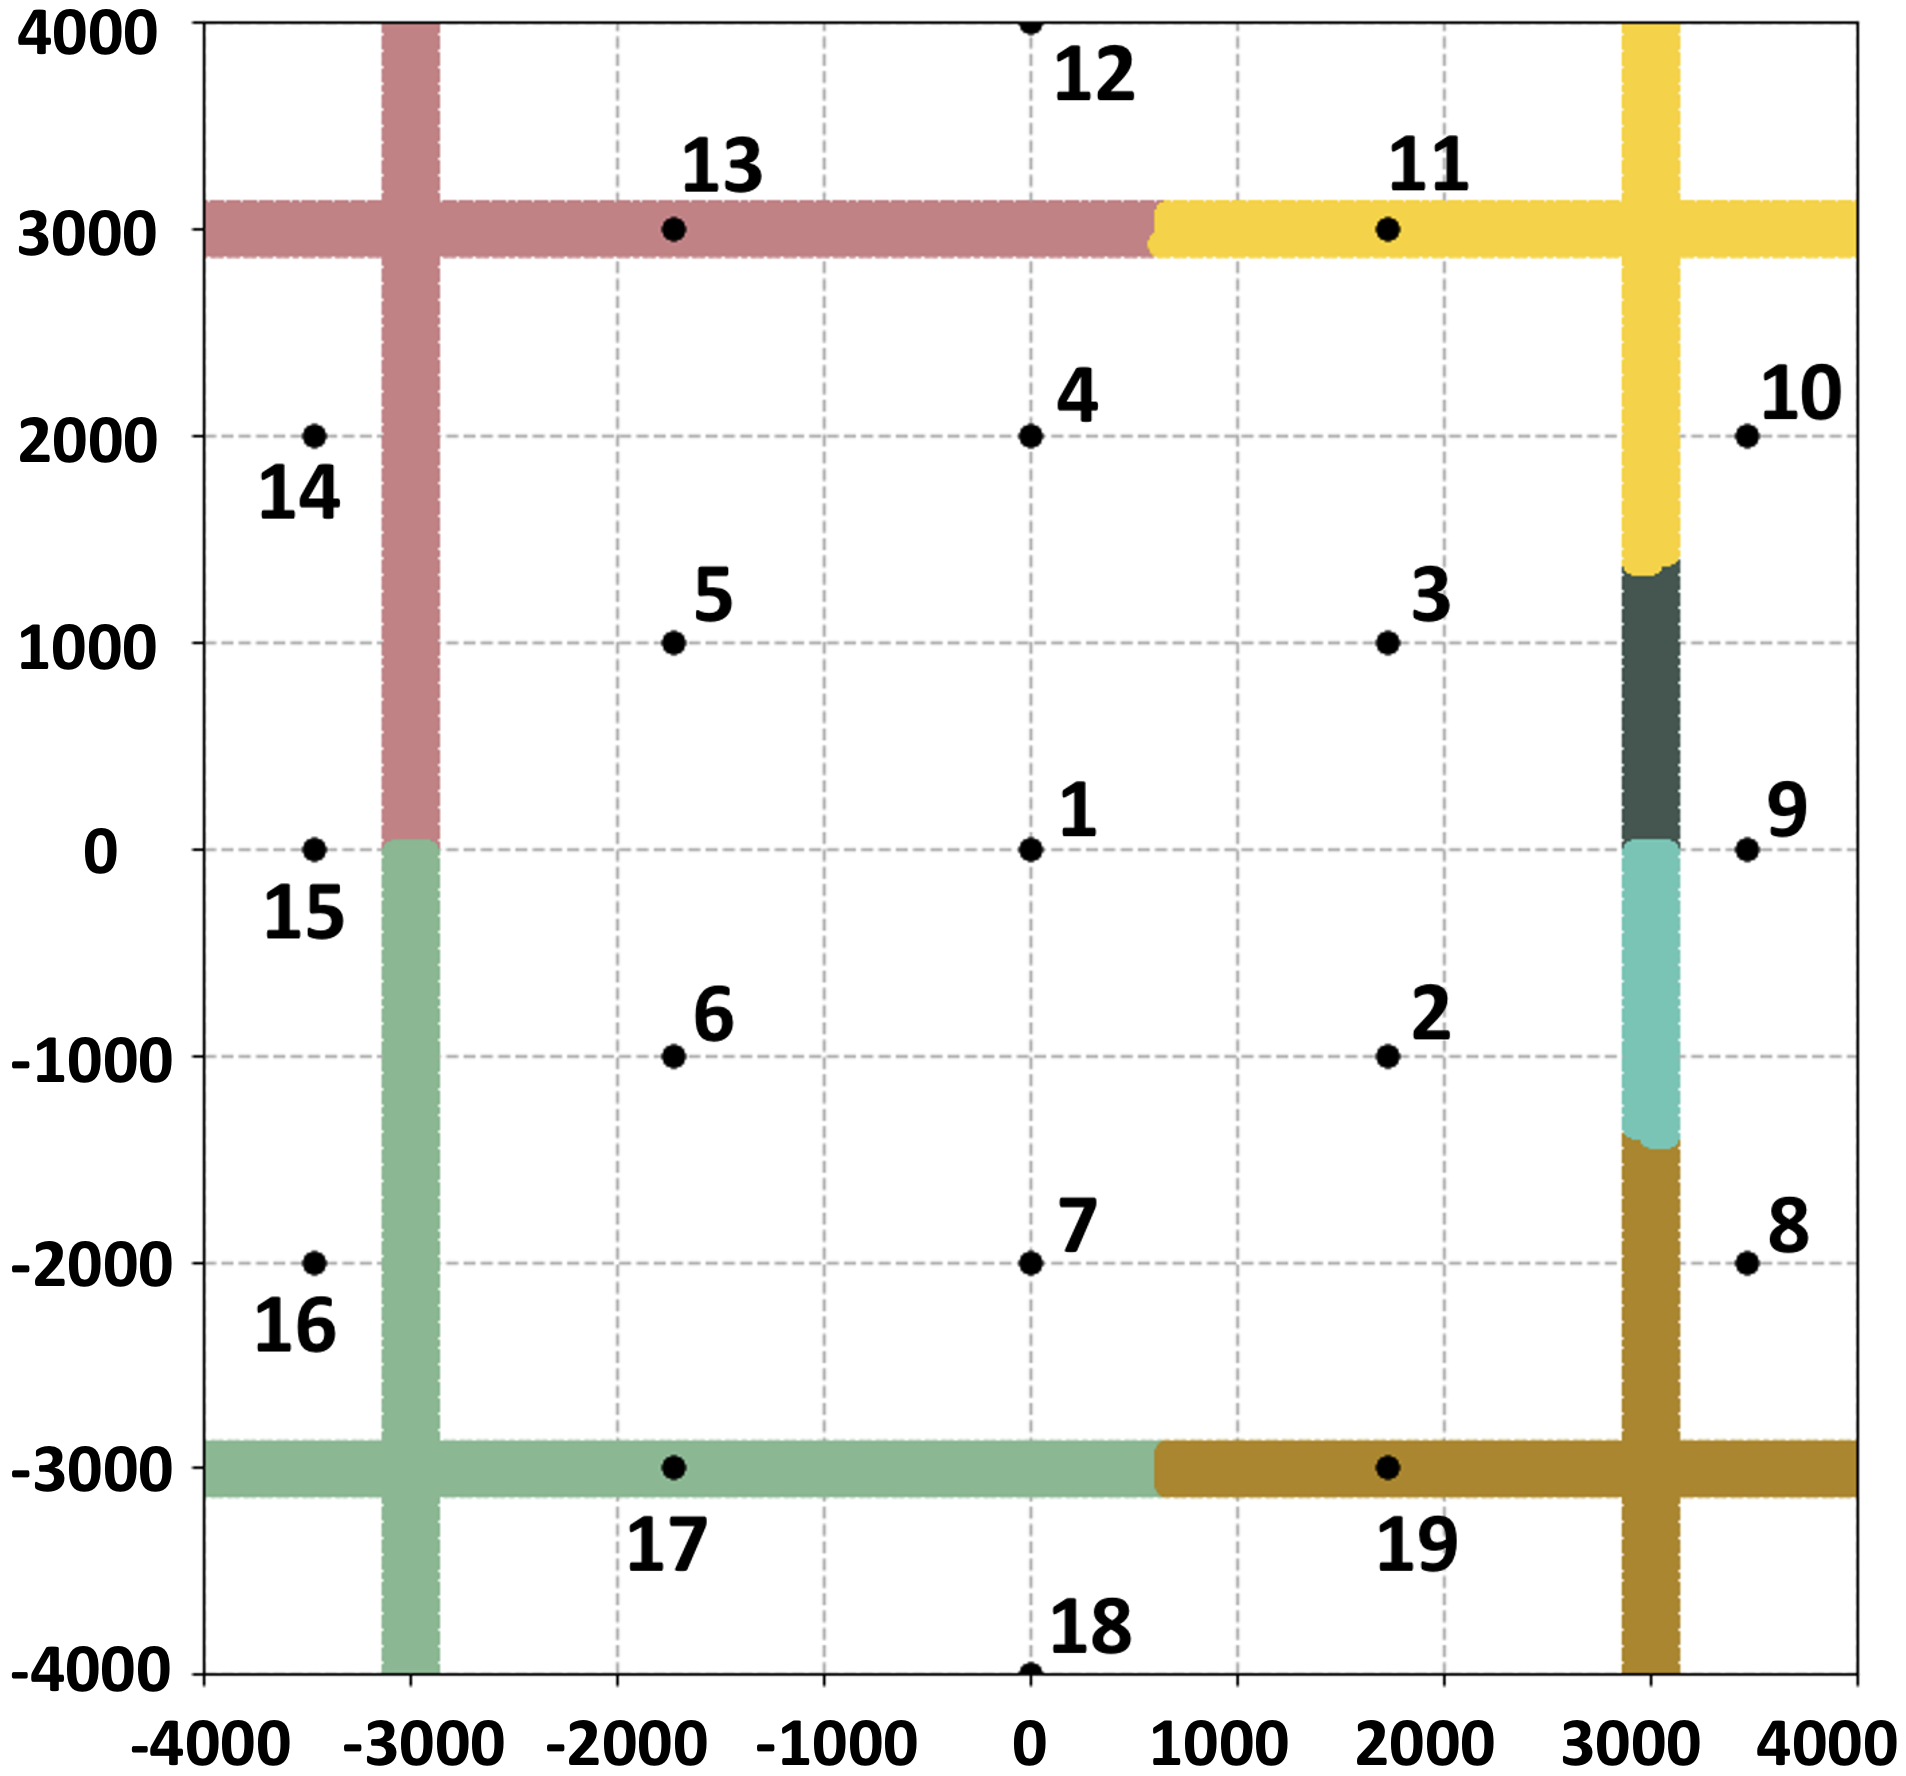
\includegraphics[width=56mm]{Figures/Exemplary-Cell-Partitioning/TWC-very-large-size-UAV-target-region-2.png}
\label{TWC-Very-Large-Size-UAV}}
\captionsetup{justification=justified}
\caption{Optimized GUEs and UAVs cell partitioning for the Max-SINR-PA-VAT algorithm with $r = 0.5$. Simulations are carried out for three different target region sizes and BS intersite distances.}
%values: \red{(1) Figs. \ref{TWC-Normal-Size-GUE} and \ref{TWC-Normal-Size-UAV} (2) Figs. \ref{TWC-Large-Size-GUE} and \ref{TWC-Large-Size-UAV} (3) Figs. \ref{TWC-Very-Large-Size-GUE} and \ref{TWC-Very-Large-Size-UAV}.}}
\label{TWC-Cell-Partitionings}
\end{figure*}


\subsection{Experimental Results}\label{Experimental-Results}

Each of the proposed algorithms is initialized with a random cell partitioning where each user at location $\bm{q}\in Q$ is assigned to a BS in a random manner. Additionally, the initial values of $\theta_n$ for all $n \in {1, \cdots, N}$ are set to $0^\circ$. In the case of the BS-VAT algorithm, which optimizes RSS  across network users, all $\rho_n$ values are set at a fixed level of $43$\,dBm. This power value is chosen because it is the straightforward optimal transmission power in the absence of interference. Conversely, for all other algorithms, the initial values of all $\rho_n$ are initialized to $0$\,dBm. The learning rate $\eta_0$ and the constant $\kappa$ are set as 0.01 and 0.999, respectively. Finally, the convergence error thresholds, $\epsilon_1$, $\epsilon_2$, and $\epsilon_3$ are chosen to be $10^{-8}$.


\begin{figure}[!t]
\centering
\subfloat[Max-RSS-VAT algorithm.]{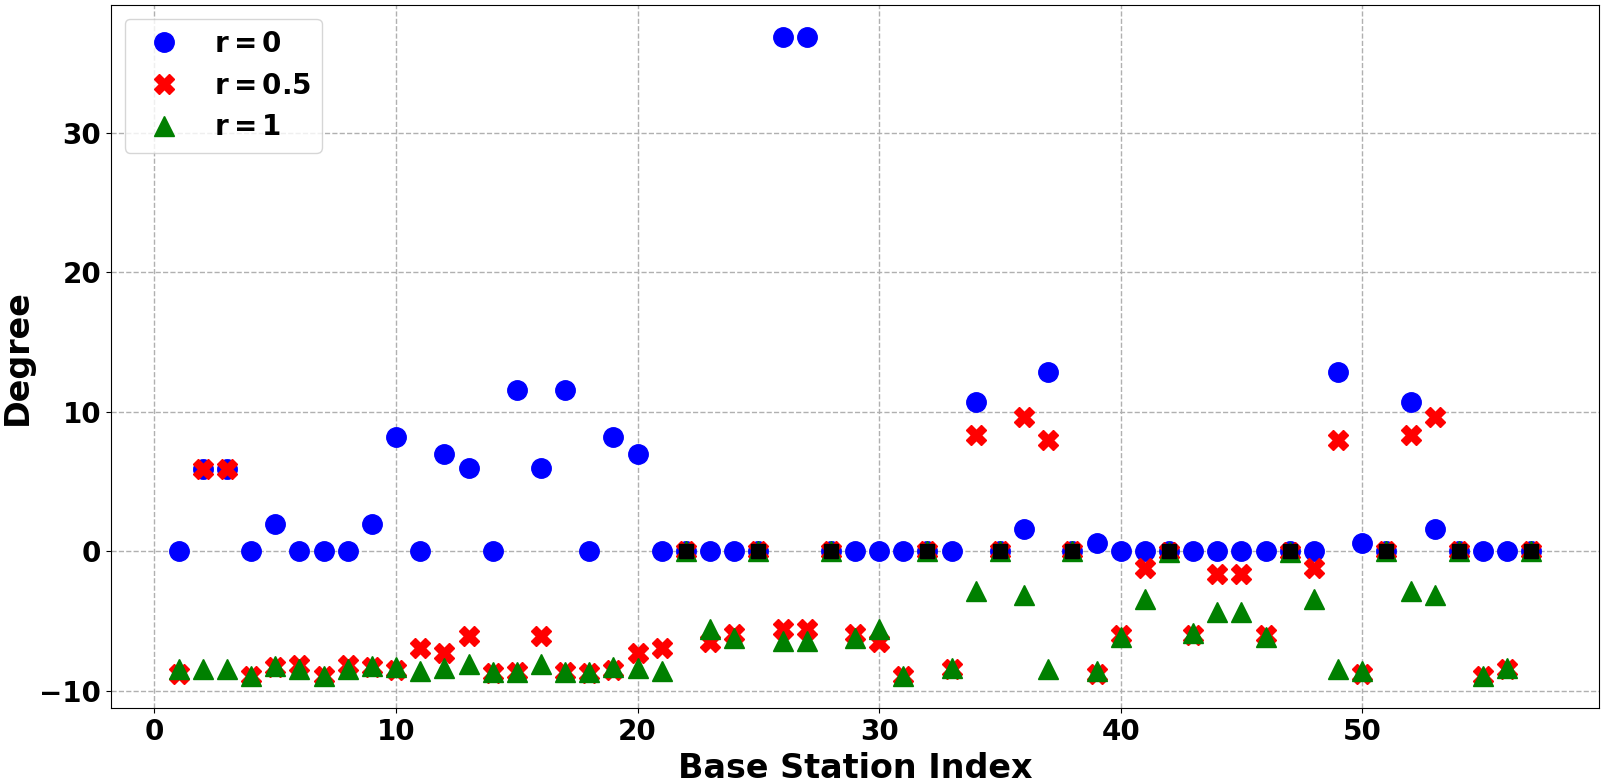
\includegraphics[width=\figwidth]{Figures/TWC-RSS-Optimal-Theta.png}
\label{TWC-RSS-Optimal-Theta}}
\hspace{0mm}\\
\vspace*{3mm}
\subfloat[MP-PA-VAT algorithm with $\mu =\nu = 0.1$.]{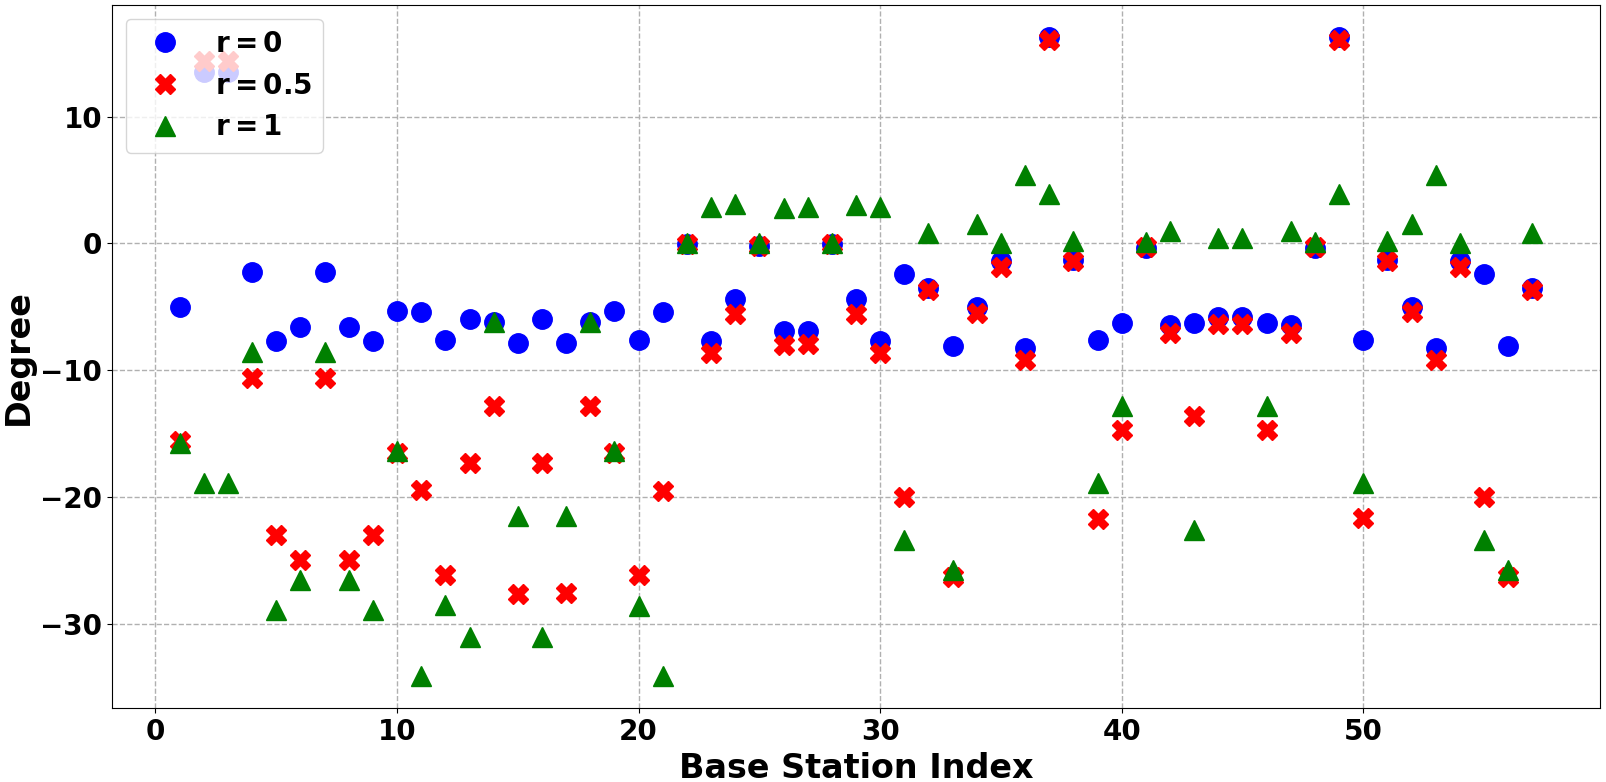
\includegraphics[width=\figwidth]{Figures/TWC-MP-010-Optimal-Theta.png}
\label{TWC-MP-010-Optimal-Theta}}
\captionsetup{justification=justified}
\caption{Optimized vertical tilts,  $\theta_i^*$: (a) Max-RSS-VAT and (b) MP-PA-VAT Algorithm with $\mu =\nu = 0.1$. Optimized for: GUEs only (green triangles, $r=1$), UAVs only (blue circles, $r=0$), and both GUEs and UAVs (red crosses, $r=0.5$).}
\label{TWC-Optimal-Theta}
\end{figure}


\subsubsection{Optimal Vertical Antenna Tilts}
Figs. \ref{TWC-RSS-Optimal-Theta} and \ref{TWC-MP-010-Optimal-Theta} display the optimal vertical antenna tilts,  $\theta_n^*$, for the Max-RSS-VAT and the MP-PA-VAT algorithms. Each figure showcases the optimal tilts for three scenarios: $r = 0$ (represented by blue circles), $r = 0.5$ (depicted by red crosses), and $r = 1$ (illustrated by green triangles). 
As anticipated, in the Max-RSS-VAT algorithm, where the BS antenna tilts are configured to optimize the average RSS across network users, prioritizing the optimization process for either ground users ($r=1$) or UAVs ($r=0$) leads to all BSs to be either downtilted or uptilted, respectively. This outcome stems from the fact that interference effects are not taken into account when the objective is to maximize the average RSS. However, in the case of $r = 0.5$, a tradeoff is achieved, resulting in a combination of uptilted and downtilted antennas. 
When it comes to the MP-PA-VAT algorithm, adjusting the vertical antenna tilts to optimize the system for any of the three scenarios ($r = 0$, $r = 0.5$, and $r = 1$) leads to a combination of uptilted and downtilted base stations. Similar observations were made for the Max-SINR-PA-VAT and SMM-PA-VAT algorithms. This is due to the fact that interference plays a substantial role in influencing the performance functions of these algorithms. In addition, in certain network configurations, certain BSs may not have an impact on the performance functions. This situation is exemplified in Fig. \ref{TWC-RSS-Optimal-Theta}, where BSs that do not contribute to the performance function in any of the three simulated scenarios ($r = 0, 0.5,$ and $1$) are depicted as black squares. 


%%%%%%%%%%%%%%%%%%%%%%%%%%%%%%%%%%%
%%%%%%%%%%%%%%%%%%%%%%%%%%%%%%%%%%%

\subsubsection{Optimal Transmission Power}
Figs. \ref{TWC-SINR-Optimal-Power} and \ref{TWC-MP-010-Optimal-Power} present the optimal transmission power values,  $\rho_n^*$, for the Max-SINR-PA-VAT and MP-PA-VAT algorithms. In each of the three scenarios, namely $r=0$, $r=0.5$, and $r=1$, a subset of BSs operates at the maximum power level of $43$\,dBm, while another subset utilizes lower power levels, and the remaining BSs are deactivated. While not shown, similar observations are made for the SMM-PA-VAT algorithm. This is in contrast to the Max-RSS-VAT algorithm where all BSs are set to the optimal transmission power value of $43$\,dBm. %This is due to the interference factor, which requires the deactivation of several BSs in order to improve the SINR performance. 
However, as the target region and ISD grow larger, the impact of interference diminishes and more BSs become active. This is demonstrated in Fig.~\ref{TWC-Cell-Partitionings} where the Max-SINR-PA-VAT algorithm is utilized to determine the most favorable network configuration for three distinct combinations of GUE and UAV target region sizes and ISD values in the case of $r = 0.5$. 
The initial pair, depicted in Figs. \ref{TWC-Normal-Size-GUE} and \ref{TWC-Normal-Size-UAV}, corresponds to the setup described in Section \ref{experimental-setup}. For the second pair, showcased in Figs. \ref{TWC-Large-Size-GUE} and \ref{TWC-Large-Size-UAV}, the GUE target region, distance between UAV corridors, and their respective widths, along with the BS ISD, are all doubled. Consequently, the optimal partitioning of the GUE target region in Fig.~\ref{TWC-Large-Size-GUE} reveals an increased number of cells and more active BSs. Finally, expanding the setup in Figs. \ref{TWC-Large-Size-GUE} and \ref{TWC-Large-Size-UAV} by an additional factor of two yields the configuration depicted in Figs. \ref{TWC-Very-Large-Size-GUE} and \ref{TWC-Very-Large-Size-UAV}. The second expansion results in a further increase in the number of cells for both the optimal GUE and UAV target region partitioning. This is primarily due to the reduced impact of interference at larger distances, allowing more BSs to efficiently serve users in their vicinity.


\begin{figure}[!t]
\centering
\subfloat[Max-SINR-PA-VAT algorithm.]{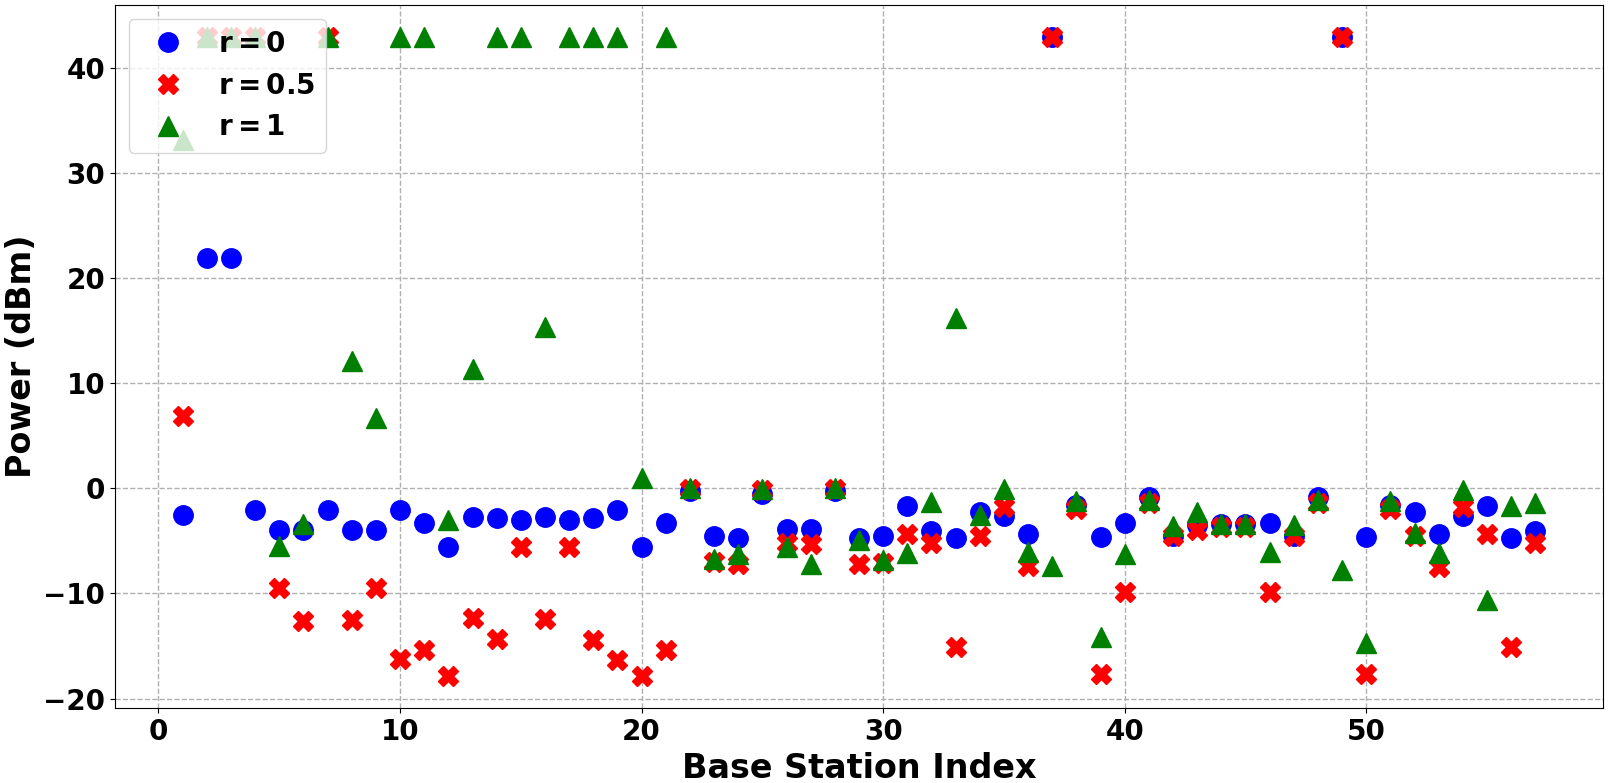
\includegraphics[width=\figwidth]{Figures/TWC-SINR-Optimal-Power.png}
\label{TWC-SINR-Optimal-Power}}
\hspace{0mm}\\
\vspace*{3mm}
\subfloat[MP-PA-VAT algorithm with $\mu =\nu = 0.1$.]{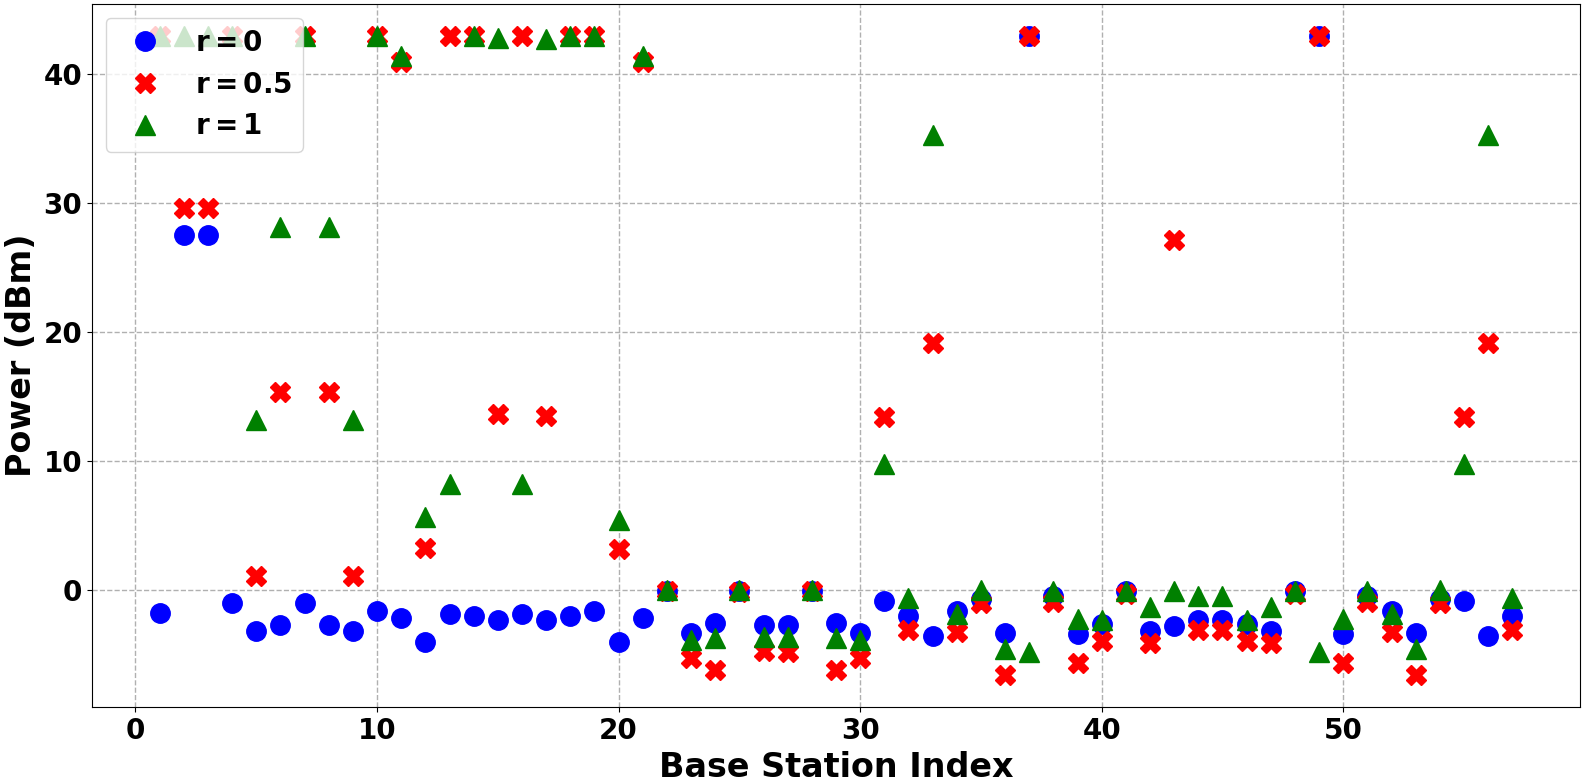
\includegraphics[width=\figwidth]{Figures/TWC-MP-010-Optimal-Power.png}
\label{TWC-MP-010-Optimal-Power}}
\captionsetup{justification=justified}
\caption{Optimized transmission powers $\rho_i^*$ for: (a) Max-SINR-PA-VAT Algorithm and (b) MP-PA-VAT Algorithm with $\mu =\nu = 0.1$. Optimized for: GUEs only (green triangles, $r=1$), UAVs only (blue circles, $r=0$), and both GUEs and UAVs (red crosses, $r=0.5$).}
\label{TWC-Optimal-Power}
\end{figure}


%%%%%%%%%%%%%%%%%%%%%%%%%%%%%%%%%%%



\begin{figure}[!t]
\centering
\subfloat[Max-RSS-VAT algorithm.]{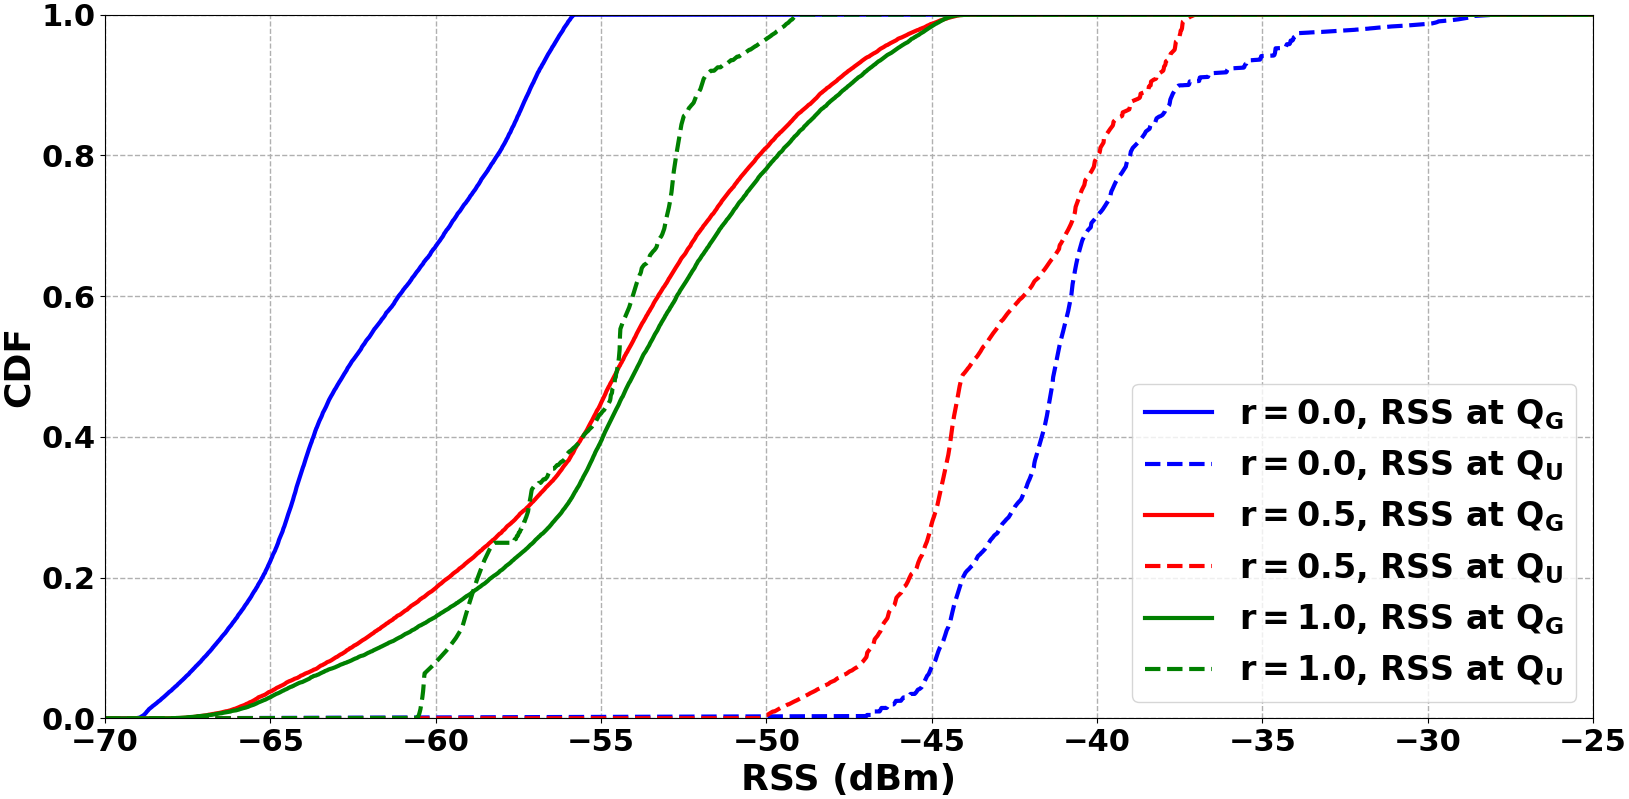
\includegraphics[width=\figwidth]{Figures/TWC-RSS-CDF-Plot.png}
\label{TWC-RSS-CDF-Plot}}
\hspace{0mm}\\
\vspace*{3mm}
\subfloat[MP-PA-VAT algorithm with $\mu =\nu = 0.1$.]{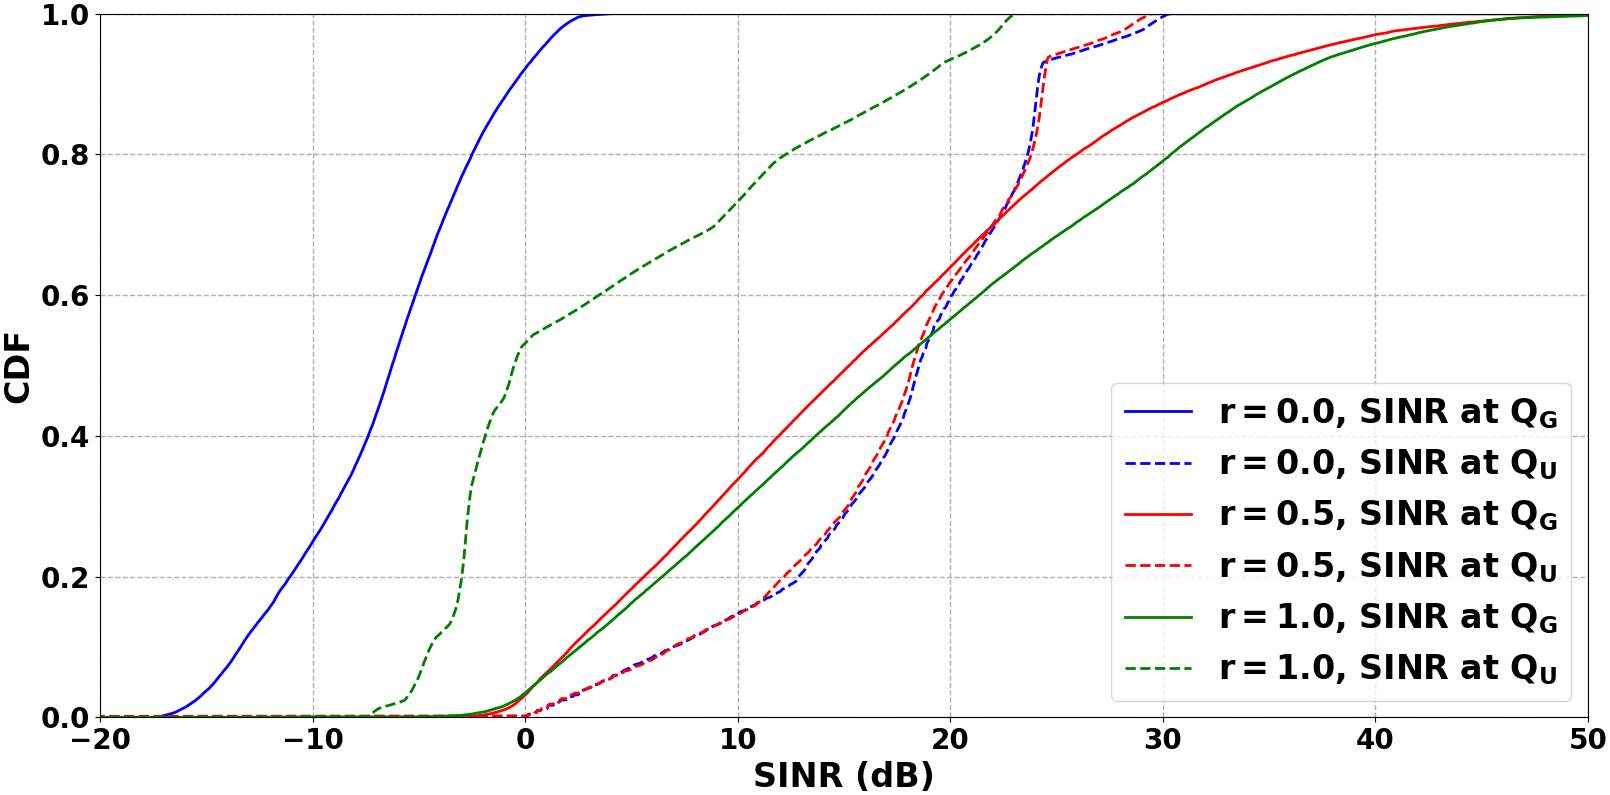
\includegraphics[width=\figwidth]{Figures/TWC-MP-010-CDF-Plot.png}
\label{TWC-MP-010-CDF-Plot}}
\hspace{0mm}\\
\vspace*{3mm}
\subfloat[Max-SINR-PA-VAT algorithm under probabilistic LoS/NLoS.]{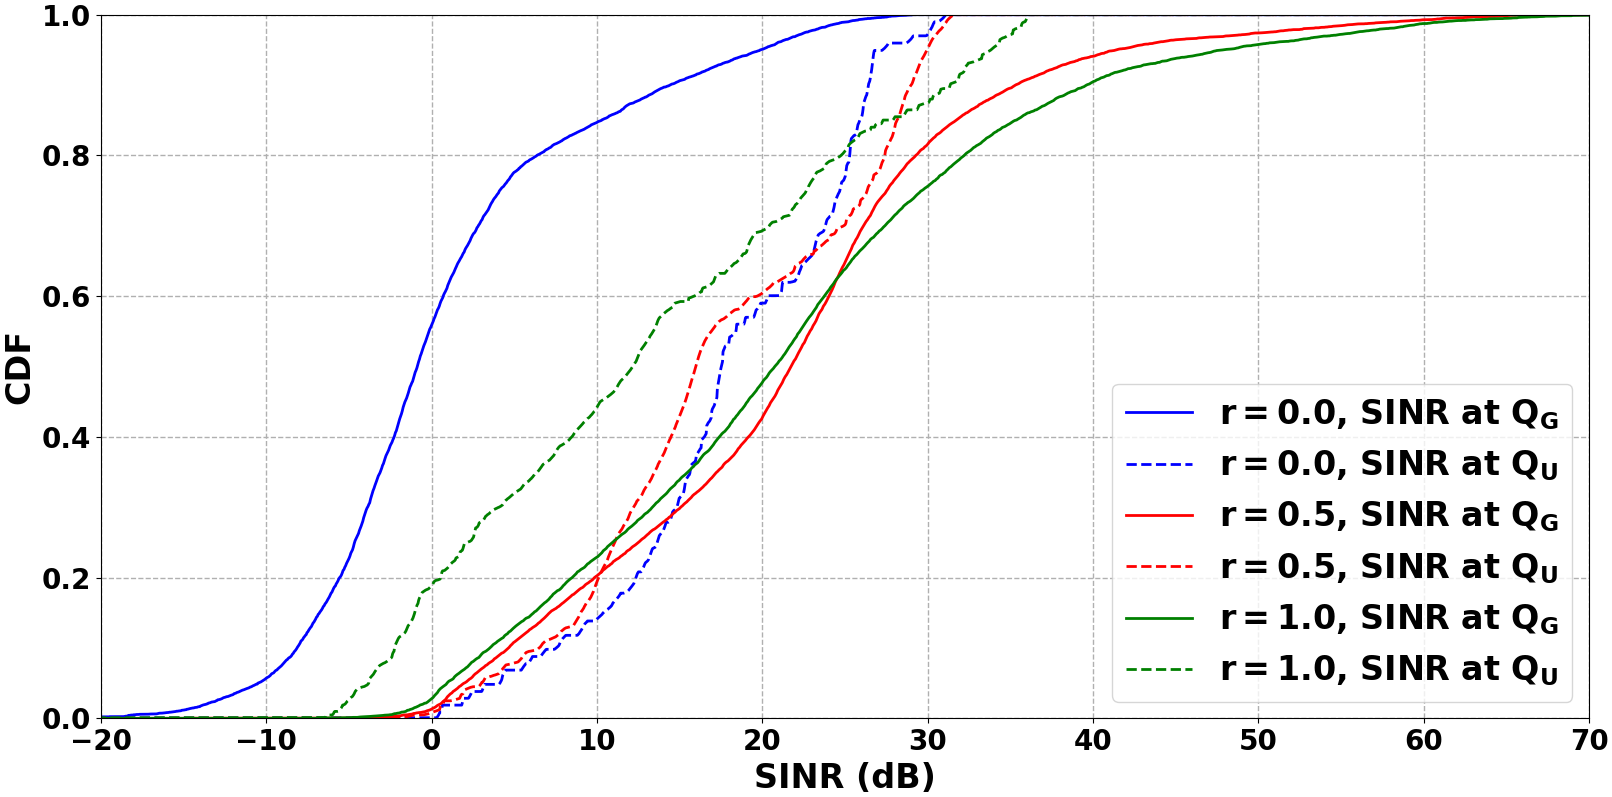
\includegraphics[width=\figwidth]{Figures/TWC-SINR-CDF-Curve-Probabilistic_LoS.png}
\label{TWC-SINR-CDF-Plot-Prob-LoS}}
\captionsetup{justification=justified}
\caption{CDF of (a) the RSS for the Max-RSS-VAT algorithm, (b) the SINR for the MP-PA-VAT algorithm with $\mu =\nu = 0.1$, and (c) the SINR for the Max-SINR-PA-VAT algorithm under probabilistic LoS/NLoS condition. Dash-dash and solid curves represent UAVs and GUEs, respectively. Three optimization scenarios are shown: GUEs only ($r=1$), UAVs only ($r=0$), and both GUEs and UAVs ($r=0.5$).}
\label{TWC-CDF-Plots}
\end{figure}
%%%%%%%%%%%%%%%%%%%%%%%%%%%%%%%%%%%

\subsubsection{Performance Improvement}\label{Resulting-performance-improvement}

% \gio{If we keep it, description of Fig.~\ref{TWC-GUE-UAV-Cells} here}
% \vspace*{1cm}


Fig. \ref{TWC-RSS-CDF-Plot} shows the cumulative distribution function (CDF) of the RSS perceived by ground users (solid line) and UAVs (dash-dash line) when the antenna tilts are optimized through the Max-RSS-VAT algorithm for ground users only ($r = 1$, green), UAVs only ($r = 0$, blue), and both ($r= 0.5$, red). Note that the ground user performance for $r = 1$ (green solid line) and the UAV performance for $r = 0$ (blue dash-dash line) can be regarded as respective upper bounds (in mean) since they entail optimizing all vertical tilts for ground users only and for UAVs only, respectively. Conversely, the ground user performance for $r = 0$ (blue solid line) and the UAV performance for $r = 1$ (green dash-dash line) can be regarded as respective baselines obtained when the vertical tilts are chosen ignoring ground users and UAVs, respectively. Fig. \ref{TWC-RSS-CDF-Plot} shows that for $r = 0.5$ the proposed Max-RSS-VAT algorithm reaches a satisfactory tradeoff by: (i) significantly boosting the RSS at UAVs (red dash-dash line) compared to the baseline (green dash-dash line) and approaching the upper bound (blue dash-dash line), and (ii) nearly preserving the RSS at ground users (red solid line) compared to the upper bound (green solid line). Specifically, the average RSS gain at UAVs amounts to $12$\,dB and comes at the expense of an average loss of only $0.7$\,dB at ground users.

Similarly, Fig. \ref{TWC-MP-010-CDF-Plot} shows the CDF of the SINR perceived by ground users and UAVs when antenna tilts and transmit power are optimized through the MP-PA-VAT algorithm with $\mu =\nu = 0.1$, for ground users only, UAVs only, and both. Fig. \ref{TWC-MP-010-CDF-Plot} shows that the proposed algorithm reaches an SINR tradeoff, boosting the average SINR at UAVs by $13$\,dB while only incurring an average loss of $2$\,dB at ground users. 
%It should be noted how, by setting $\mu =\nu = 0.1$, the proposed algorithm ensures fairness among users, with 95\% of all UAVs and ground users experiencing SINRs above \mynote{WW~dB} and \mynote{ZZ~dB}, respectively.





\begin{comment}
\begin{figure}[!t]
\centering
\subfloat[Setup as per Sec.~\ref{experimental-setup}.]{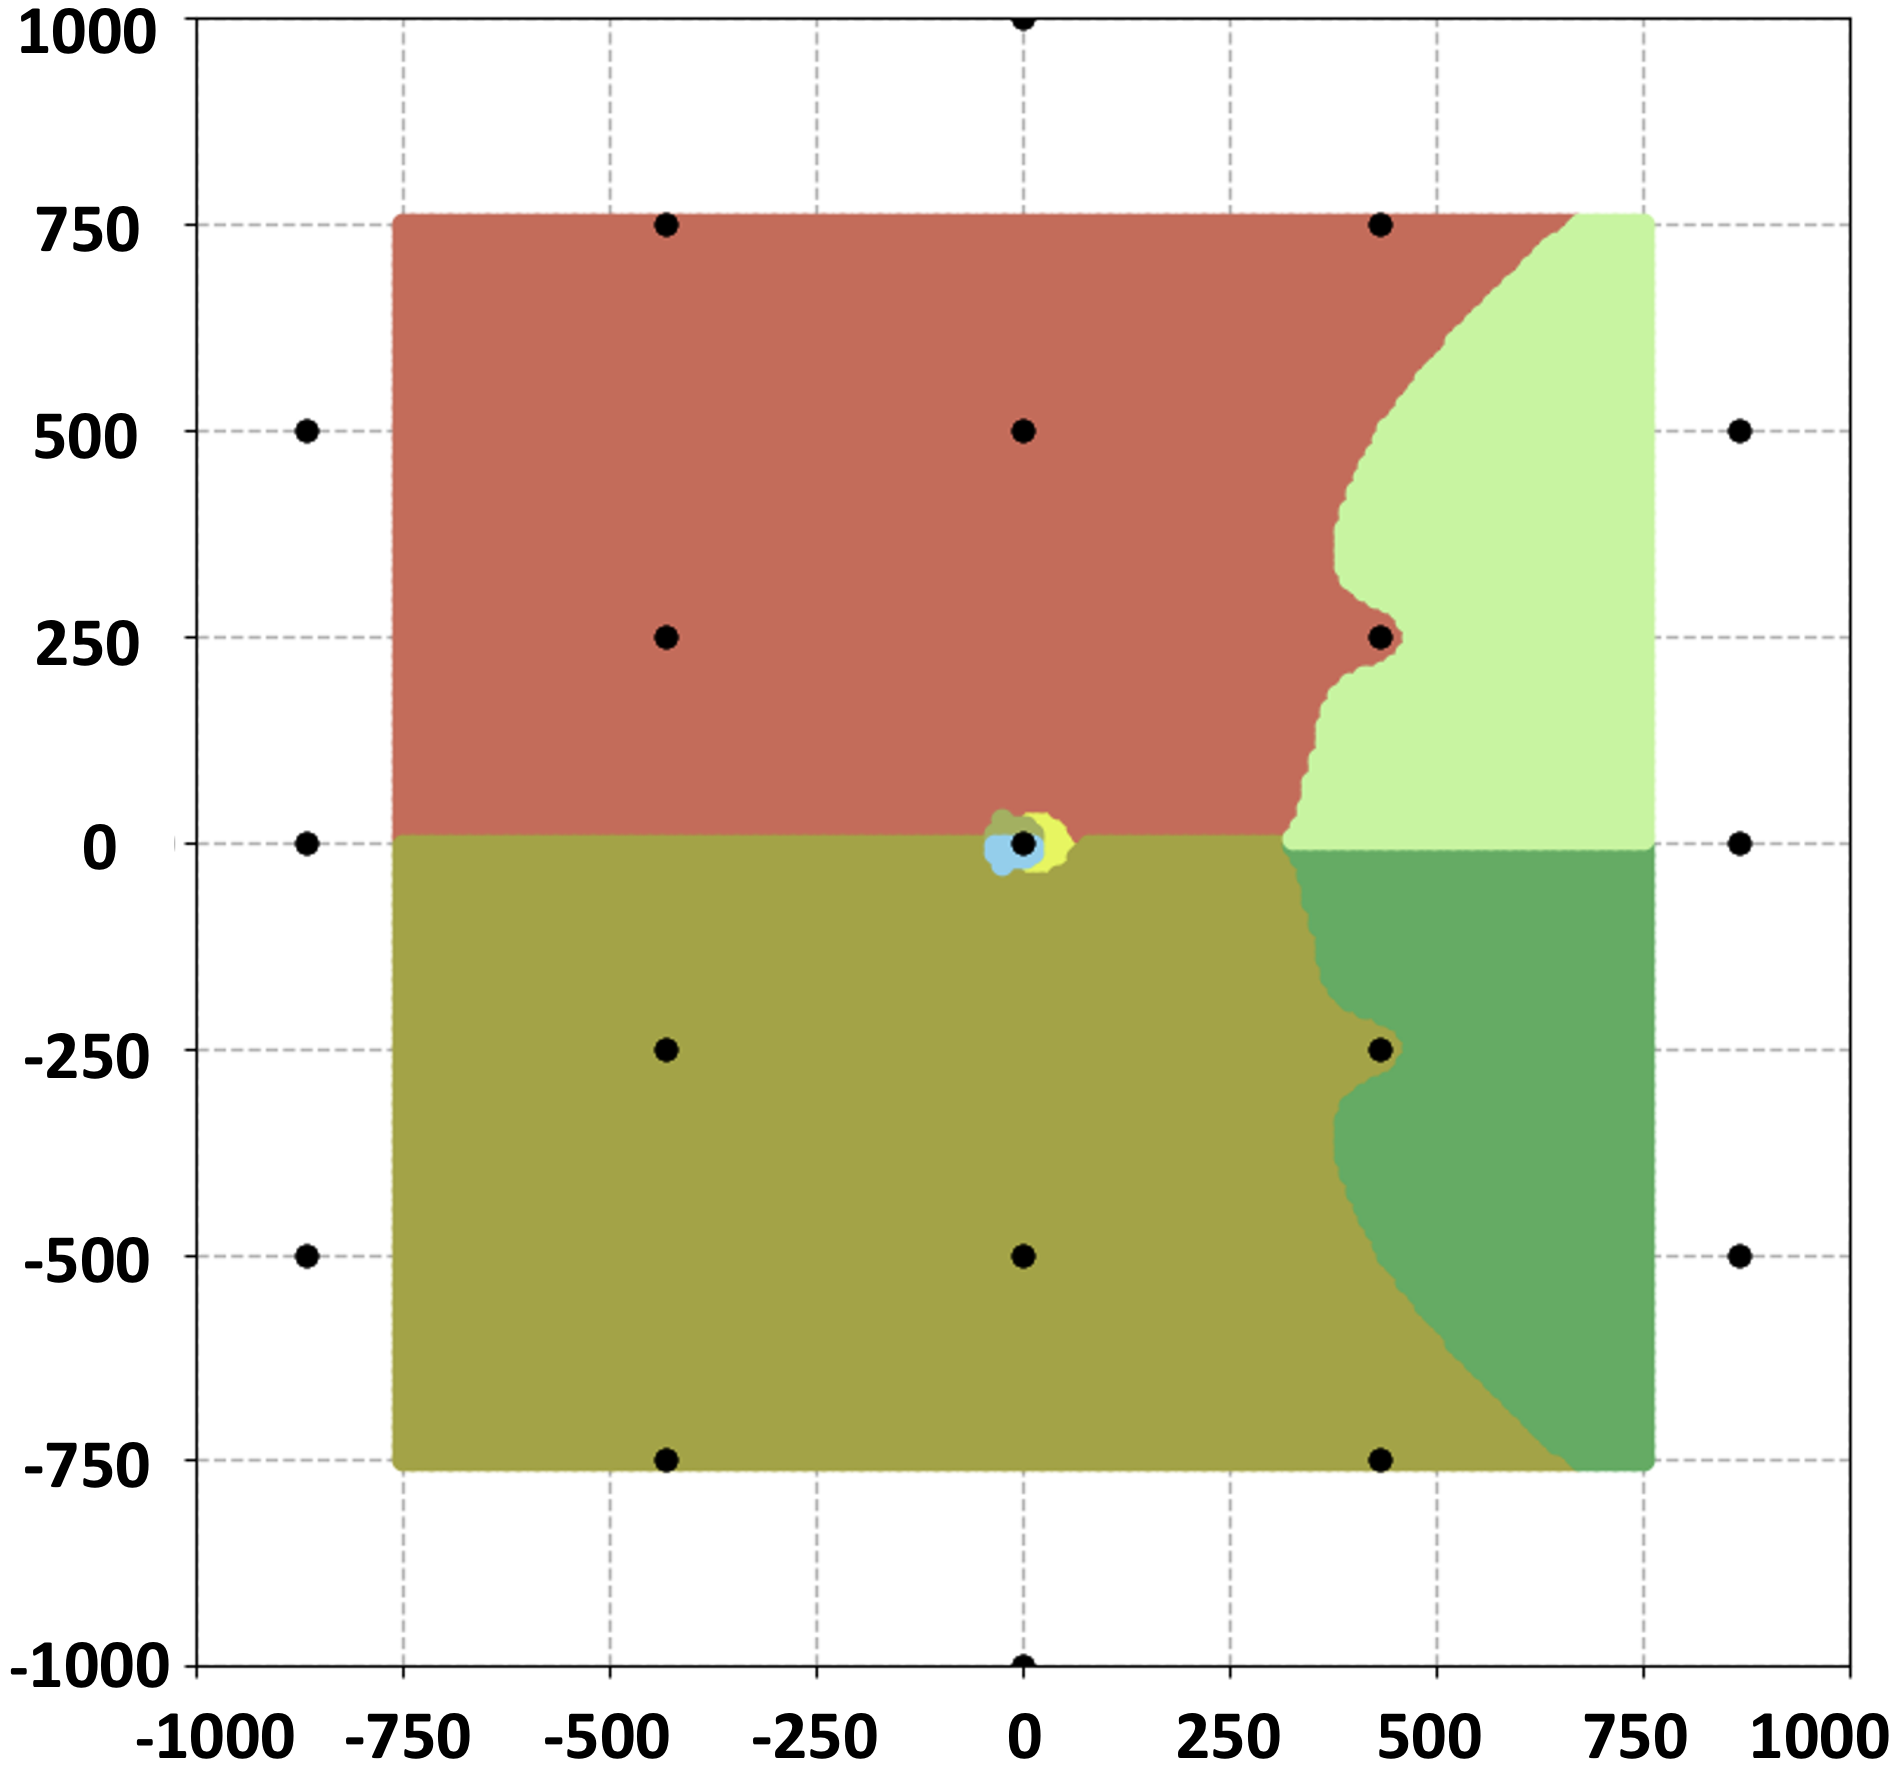
\includegraphics[width=42mm]{Figures/Exemplary-Cell-Partitioning/TWC-normal-size-SINR-GUE-Cells_1.png}
\label{TWC-Normal-Size-GUE}}
\hspace{0mm}
\subfloat[Setup as per Sec.~\ref{experimental-setup}.]{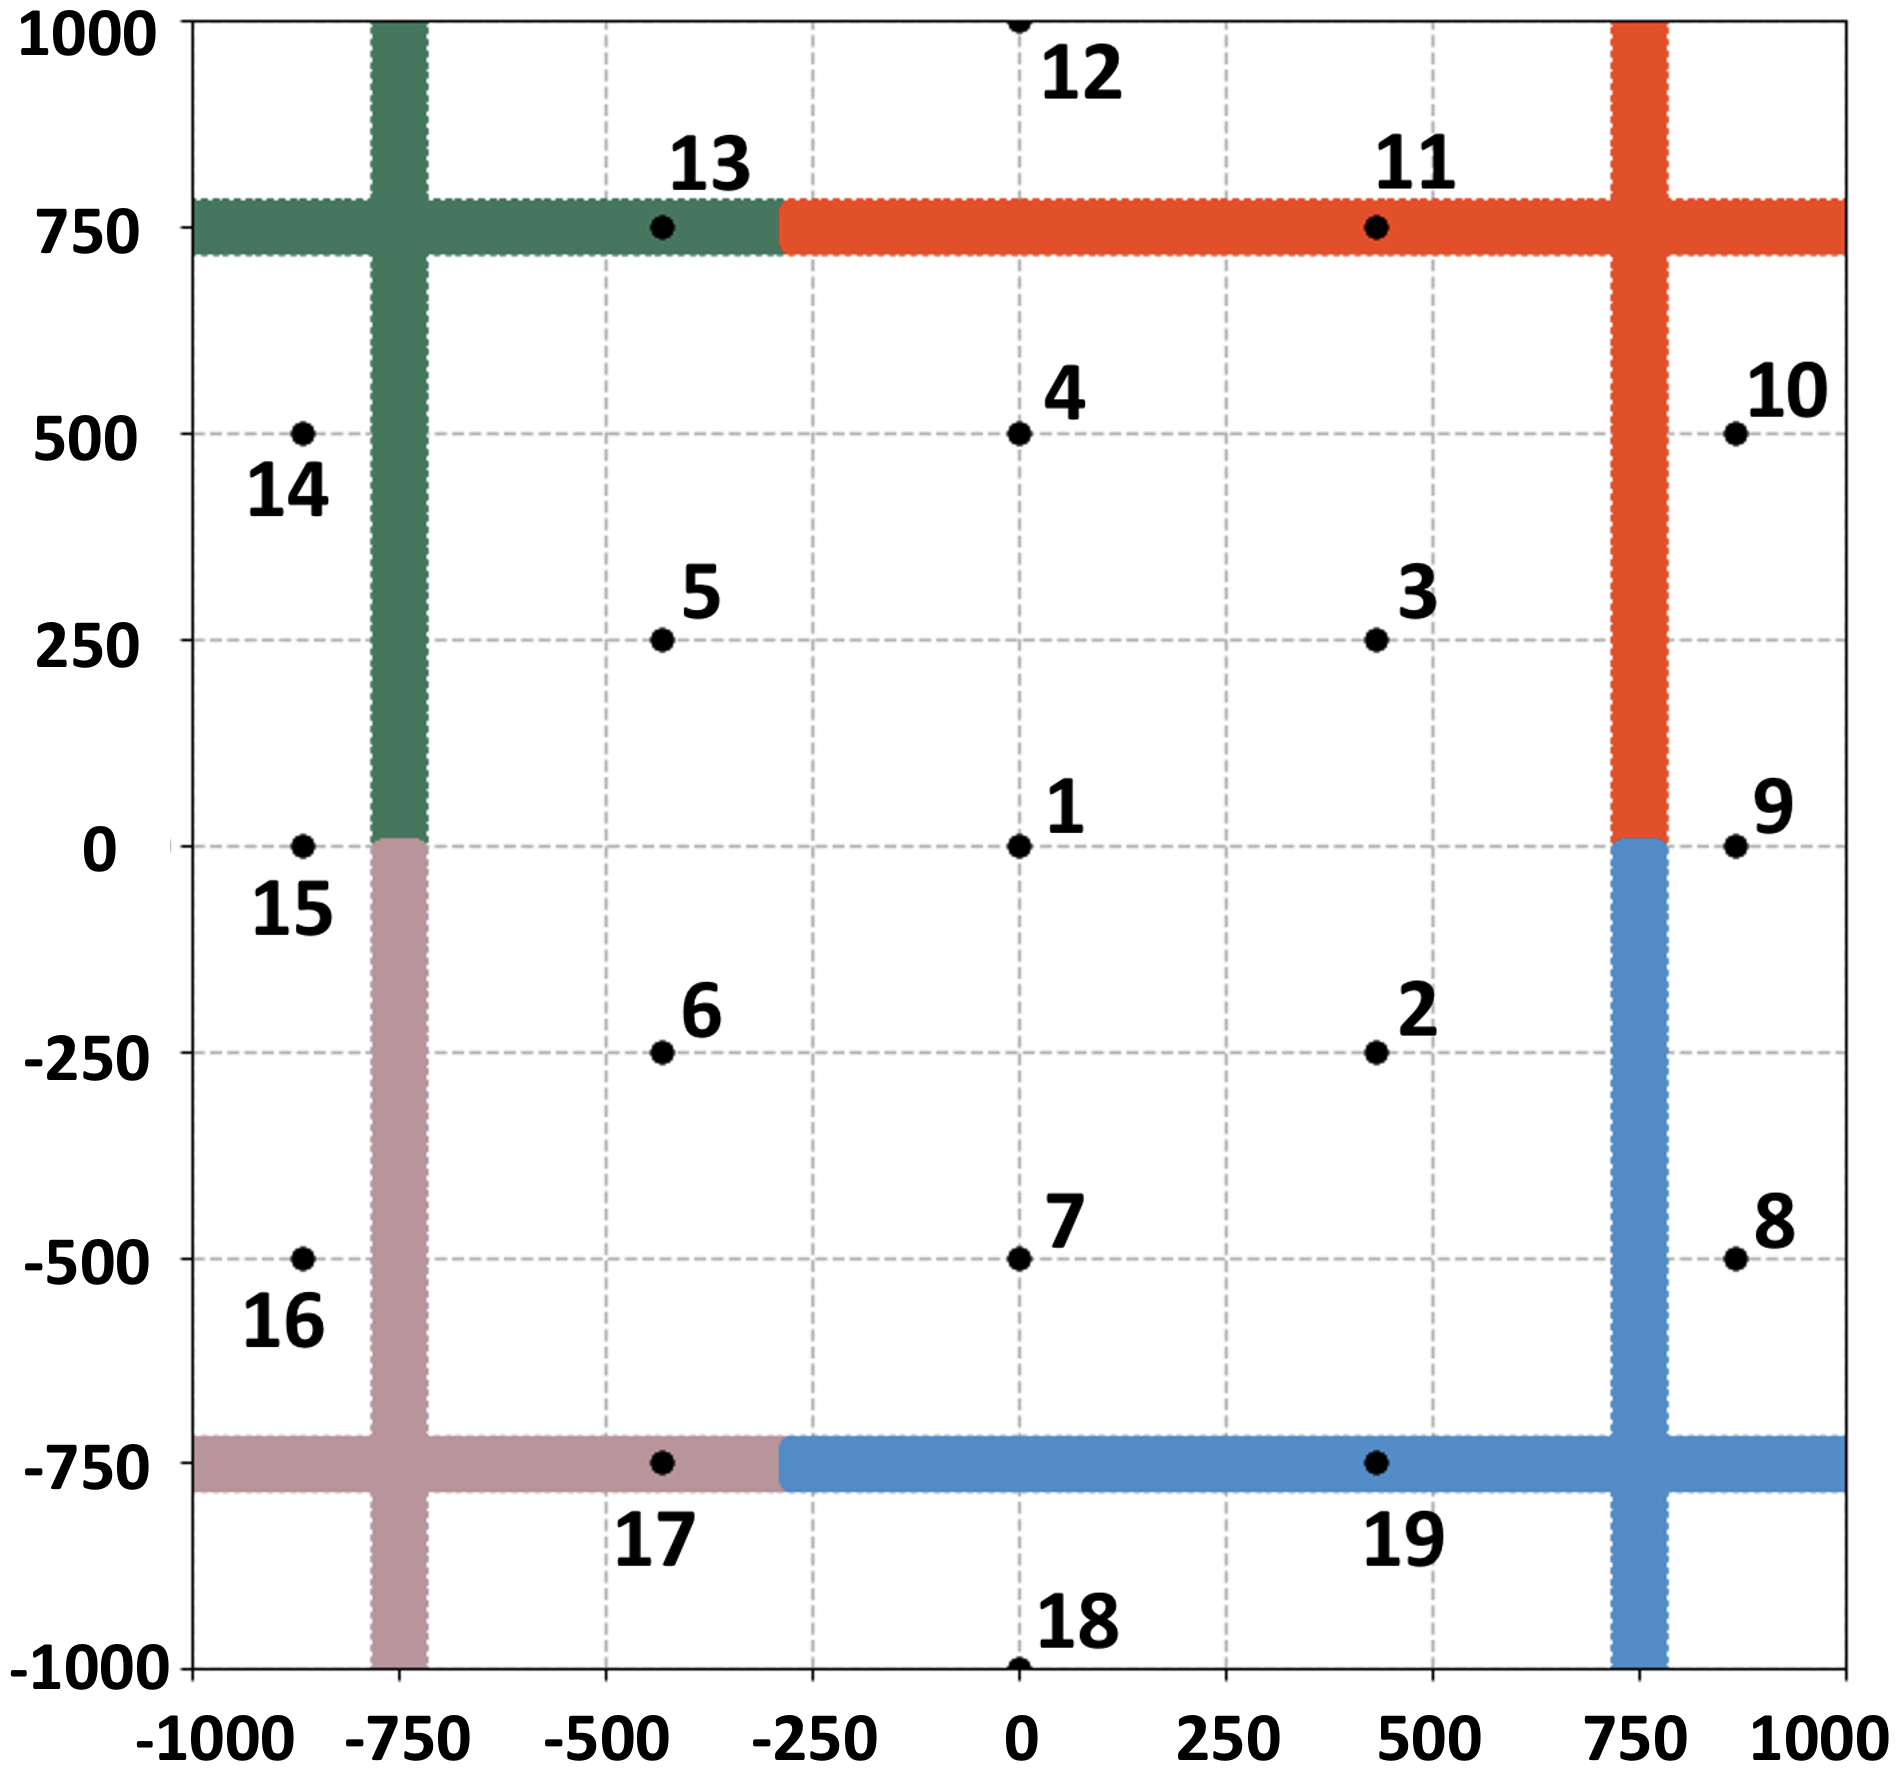
\includegraphics[width=42mm]{Figures/Exemplary-Cell-Partitioning/TWC-normal-size-UAV-target-region.png}
\label{TWC-Normal-Size-UAV}}
\hspace{0mm}\\
\vspace*{3mm}
\subfloat[Setup as per Sec.~\ref{experimental-setup} $\times$2.]{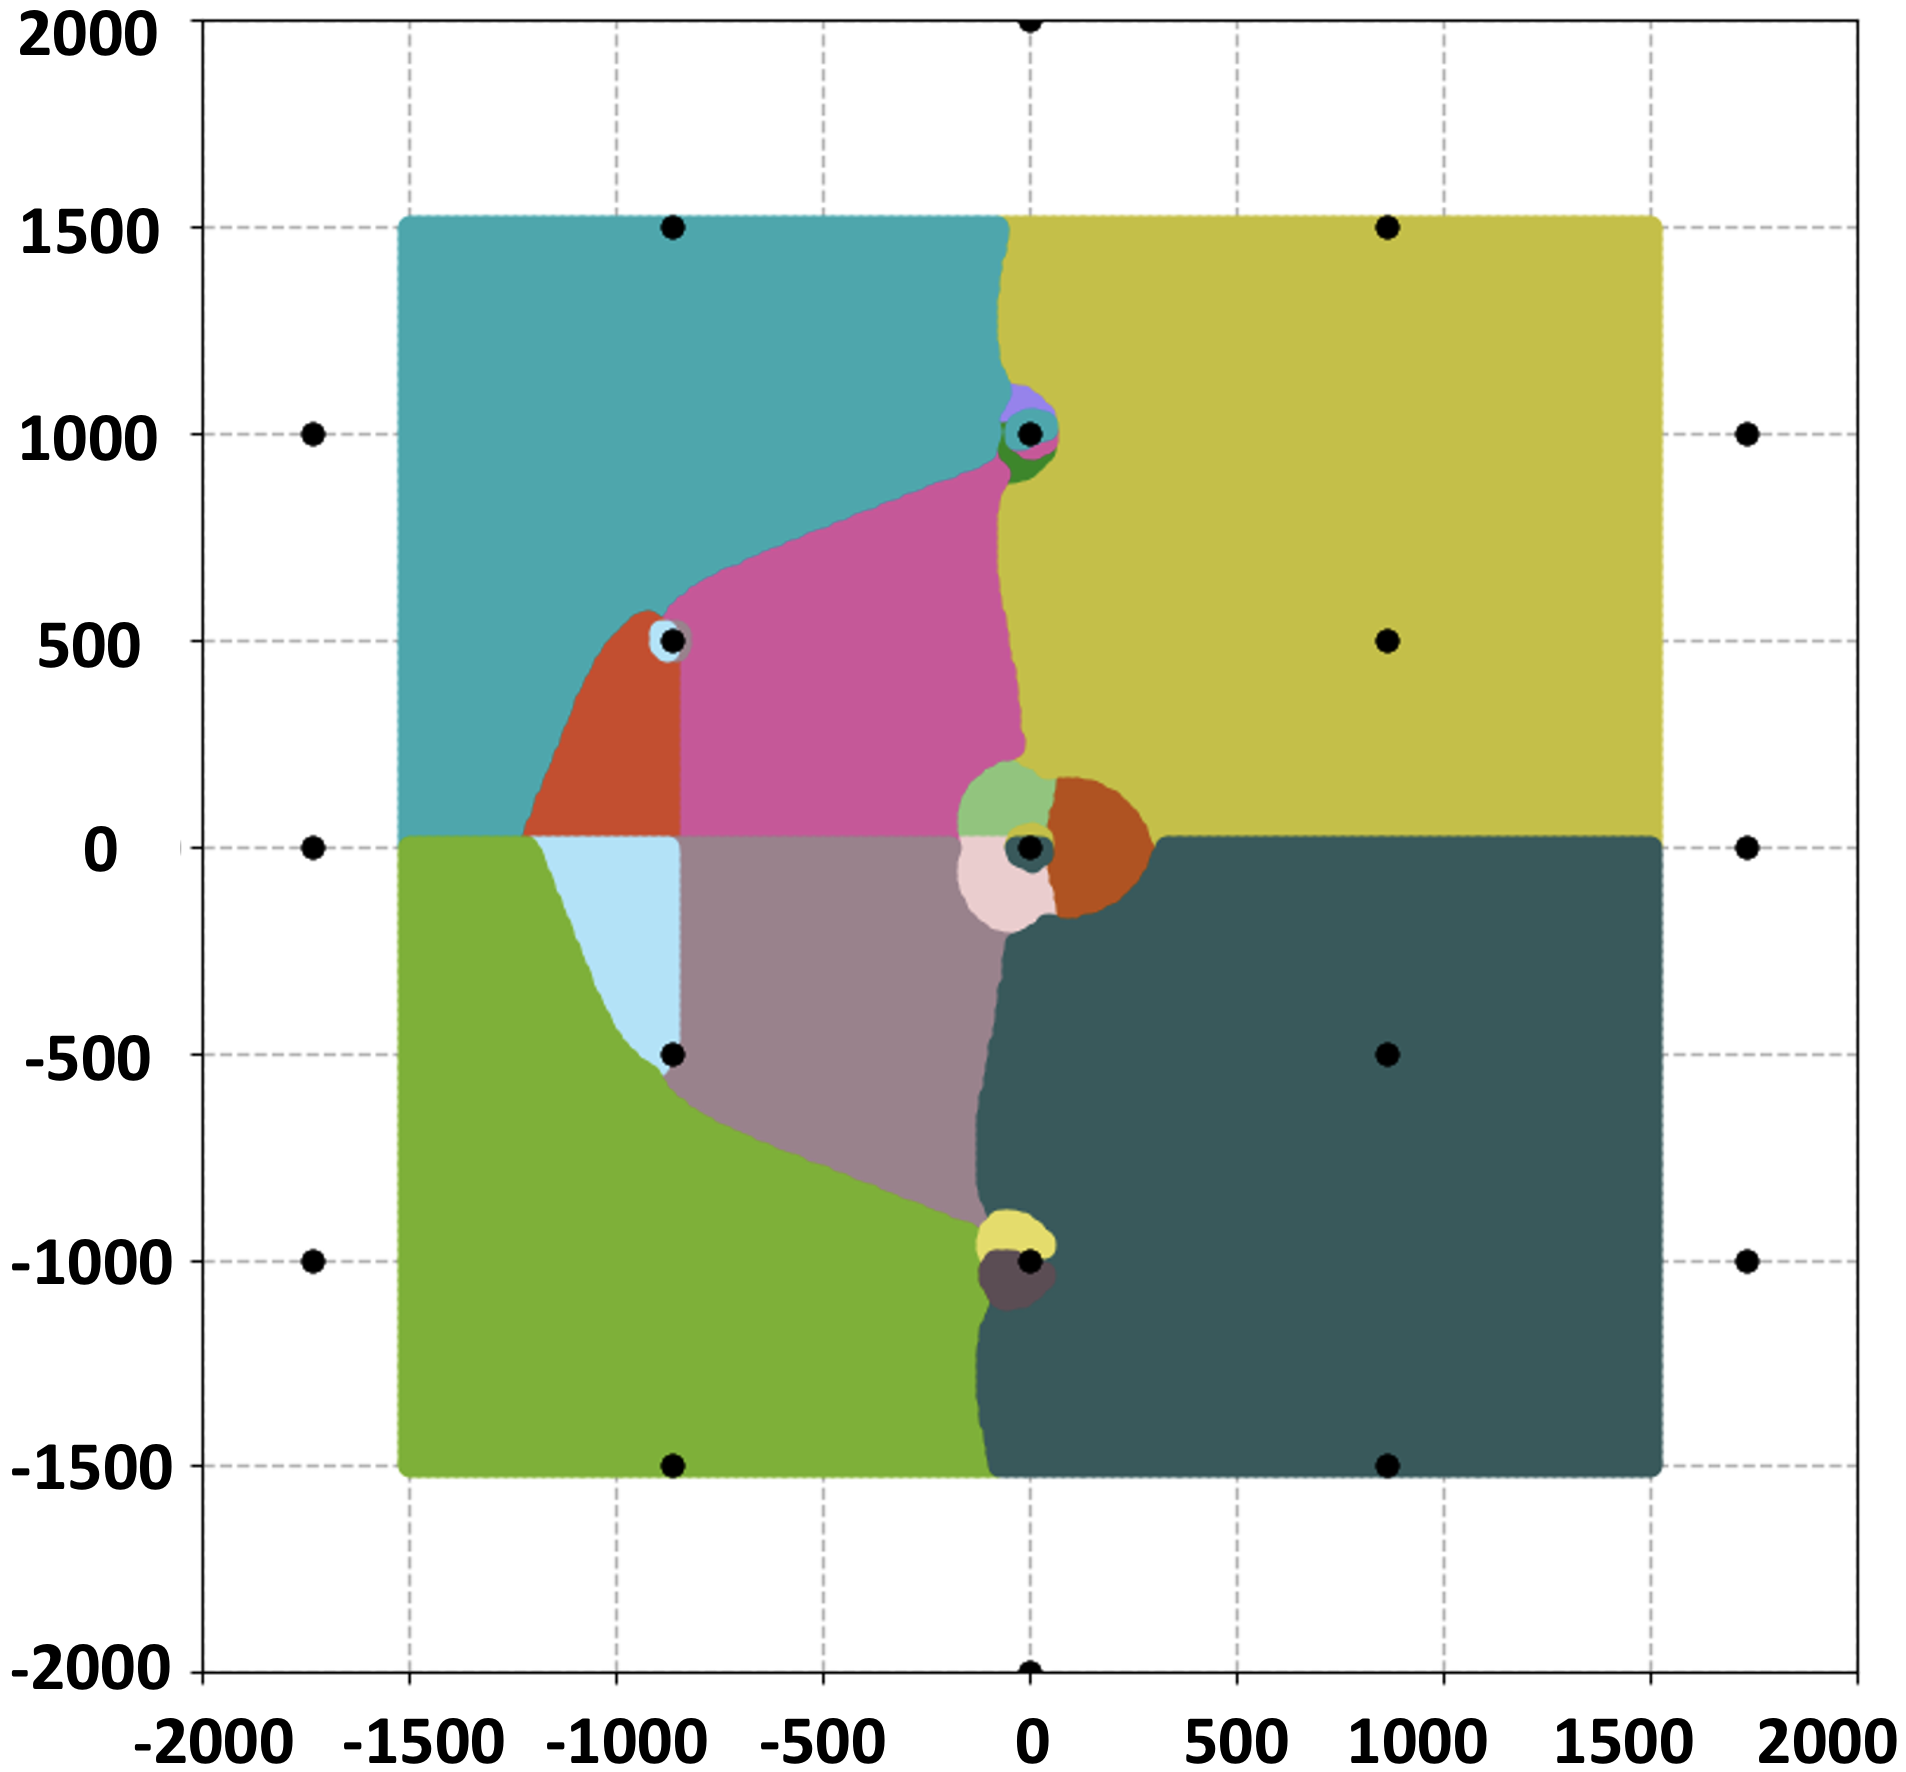
\includegraphics[width=42mm]{Figures/Exemplary-Cell-Partitioning/TWC-SINR-GUE-Large-Cells_4.png}
\label{TWC-Large-Size-GUE}}
\hspace{0mm}
\subfloat[Setup as per Sec.~\ref{experimental-setup} $\times$2.]{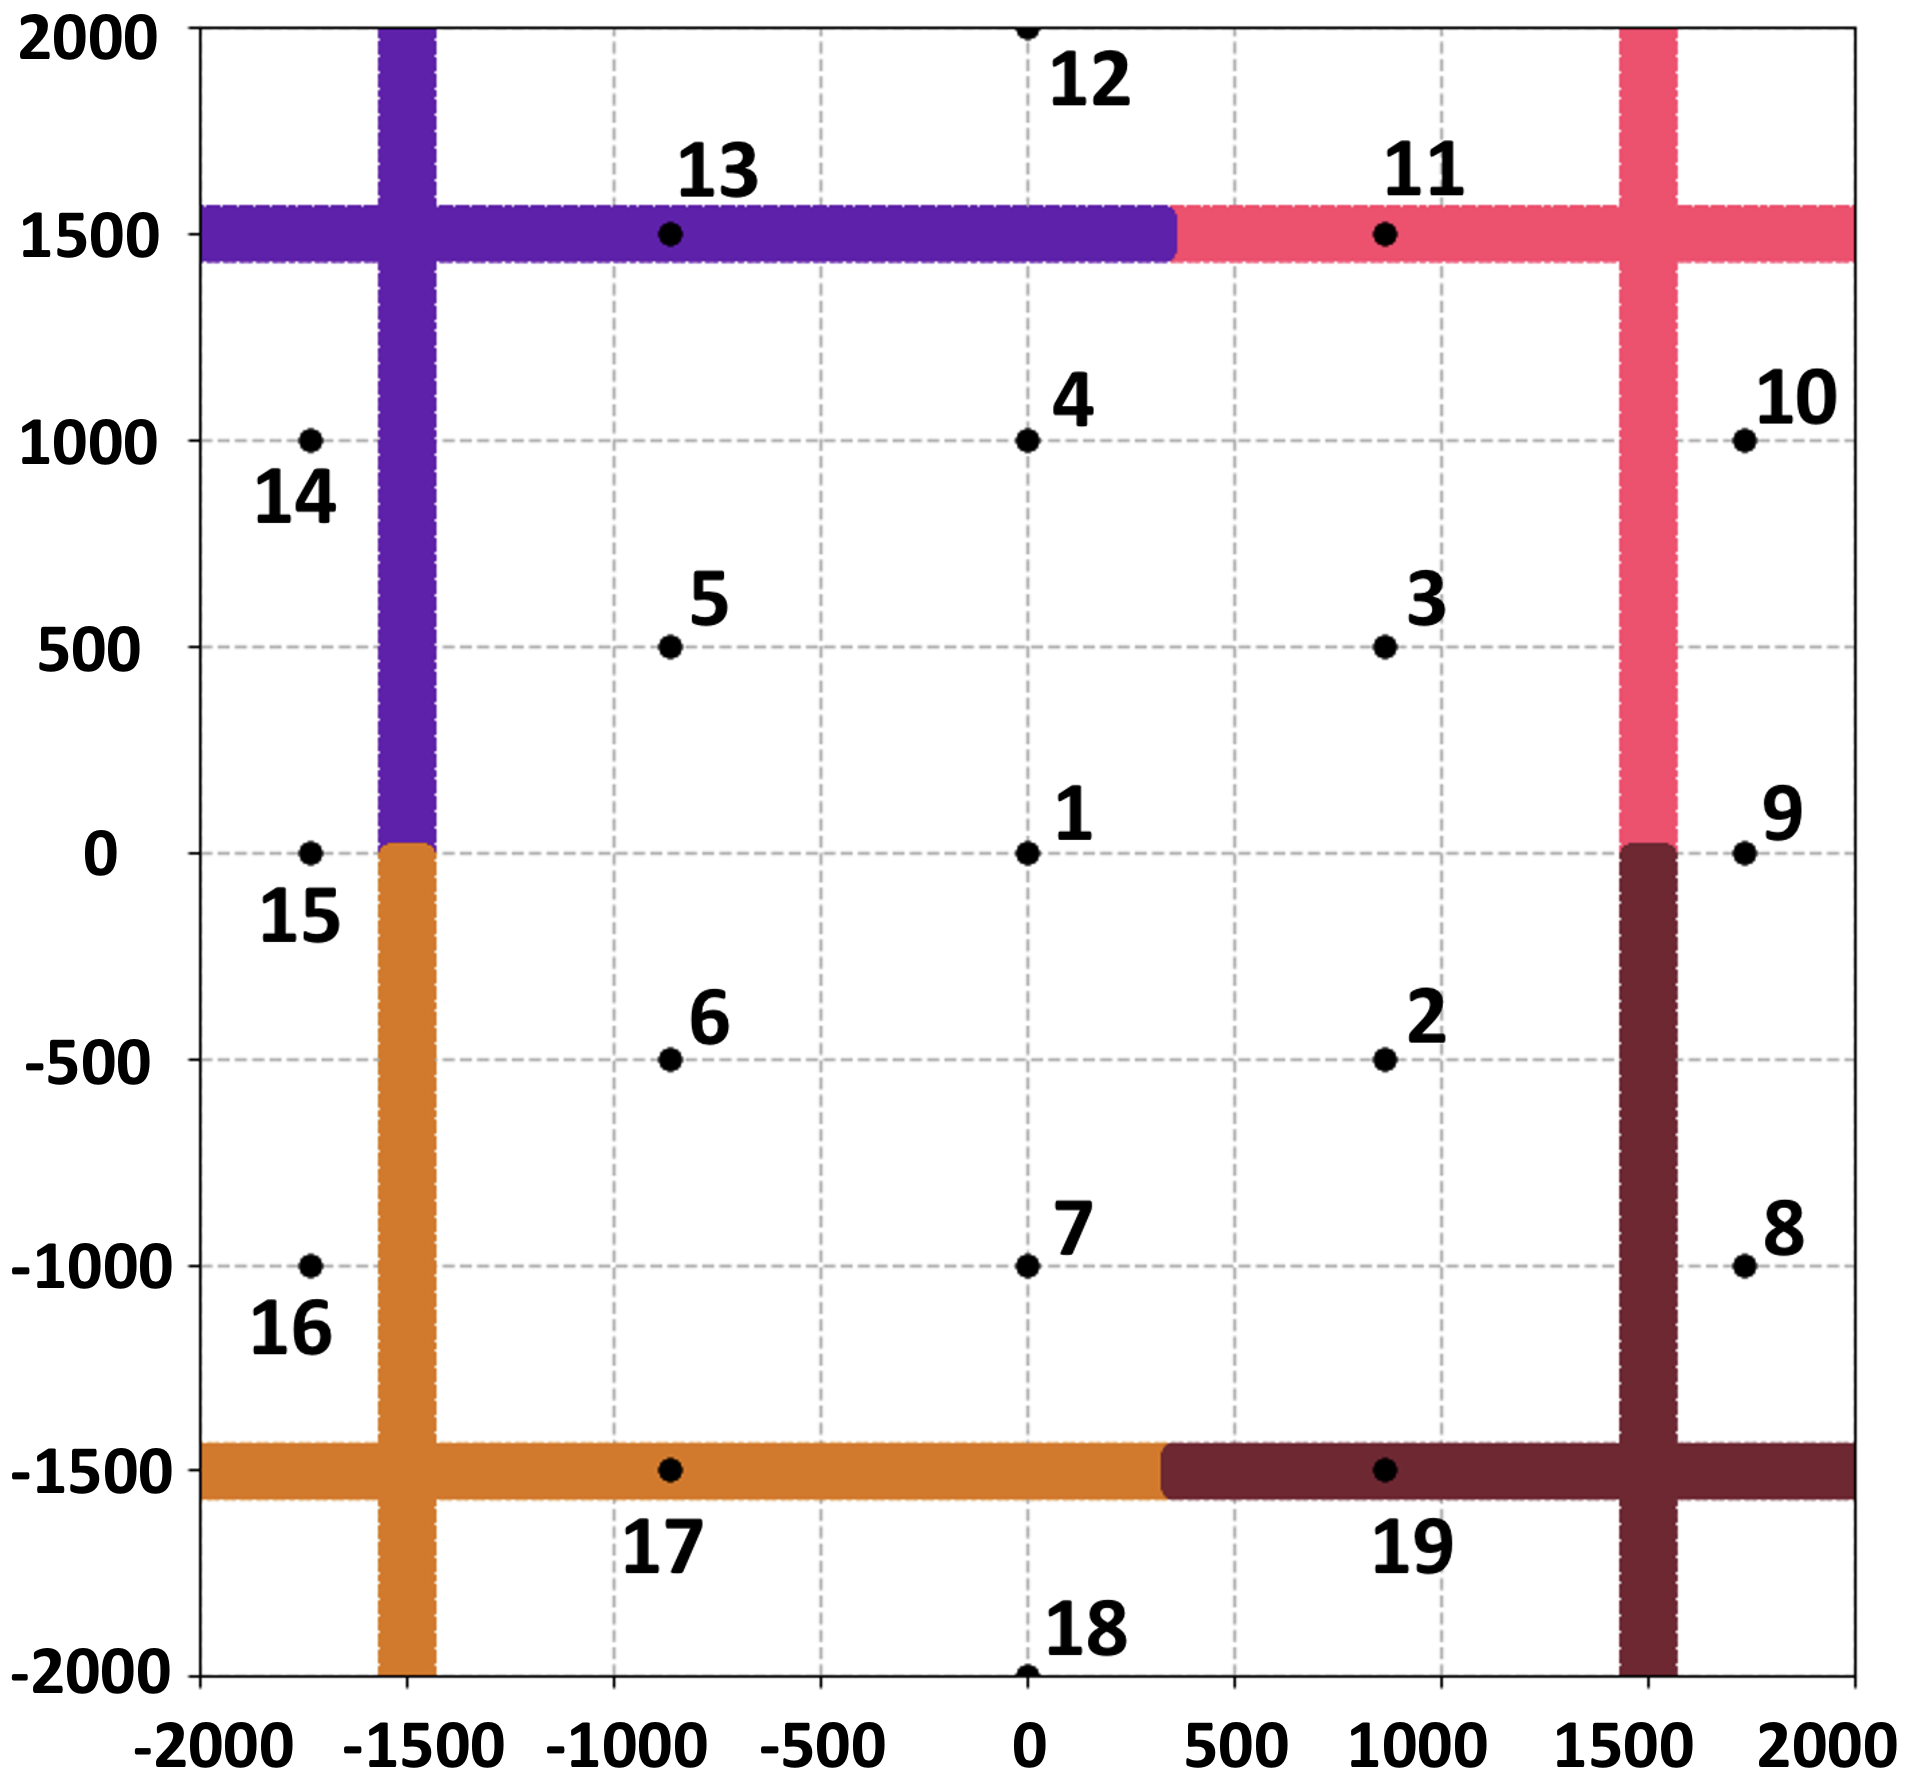
\includegraphics[width=42mm]{Figures/Exemplary-Cell-Partitioning/TWC-large-size-UAV-target-region-2.png}
\label{TWC-Large-Size-UAV}}
\hspace{0mm}\\
\vspace*{3mm}
\subfloat[Setup as per Sec.~\ref{experimental-setup} $\times$4.]{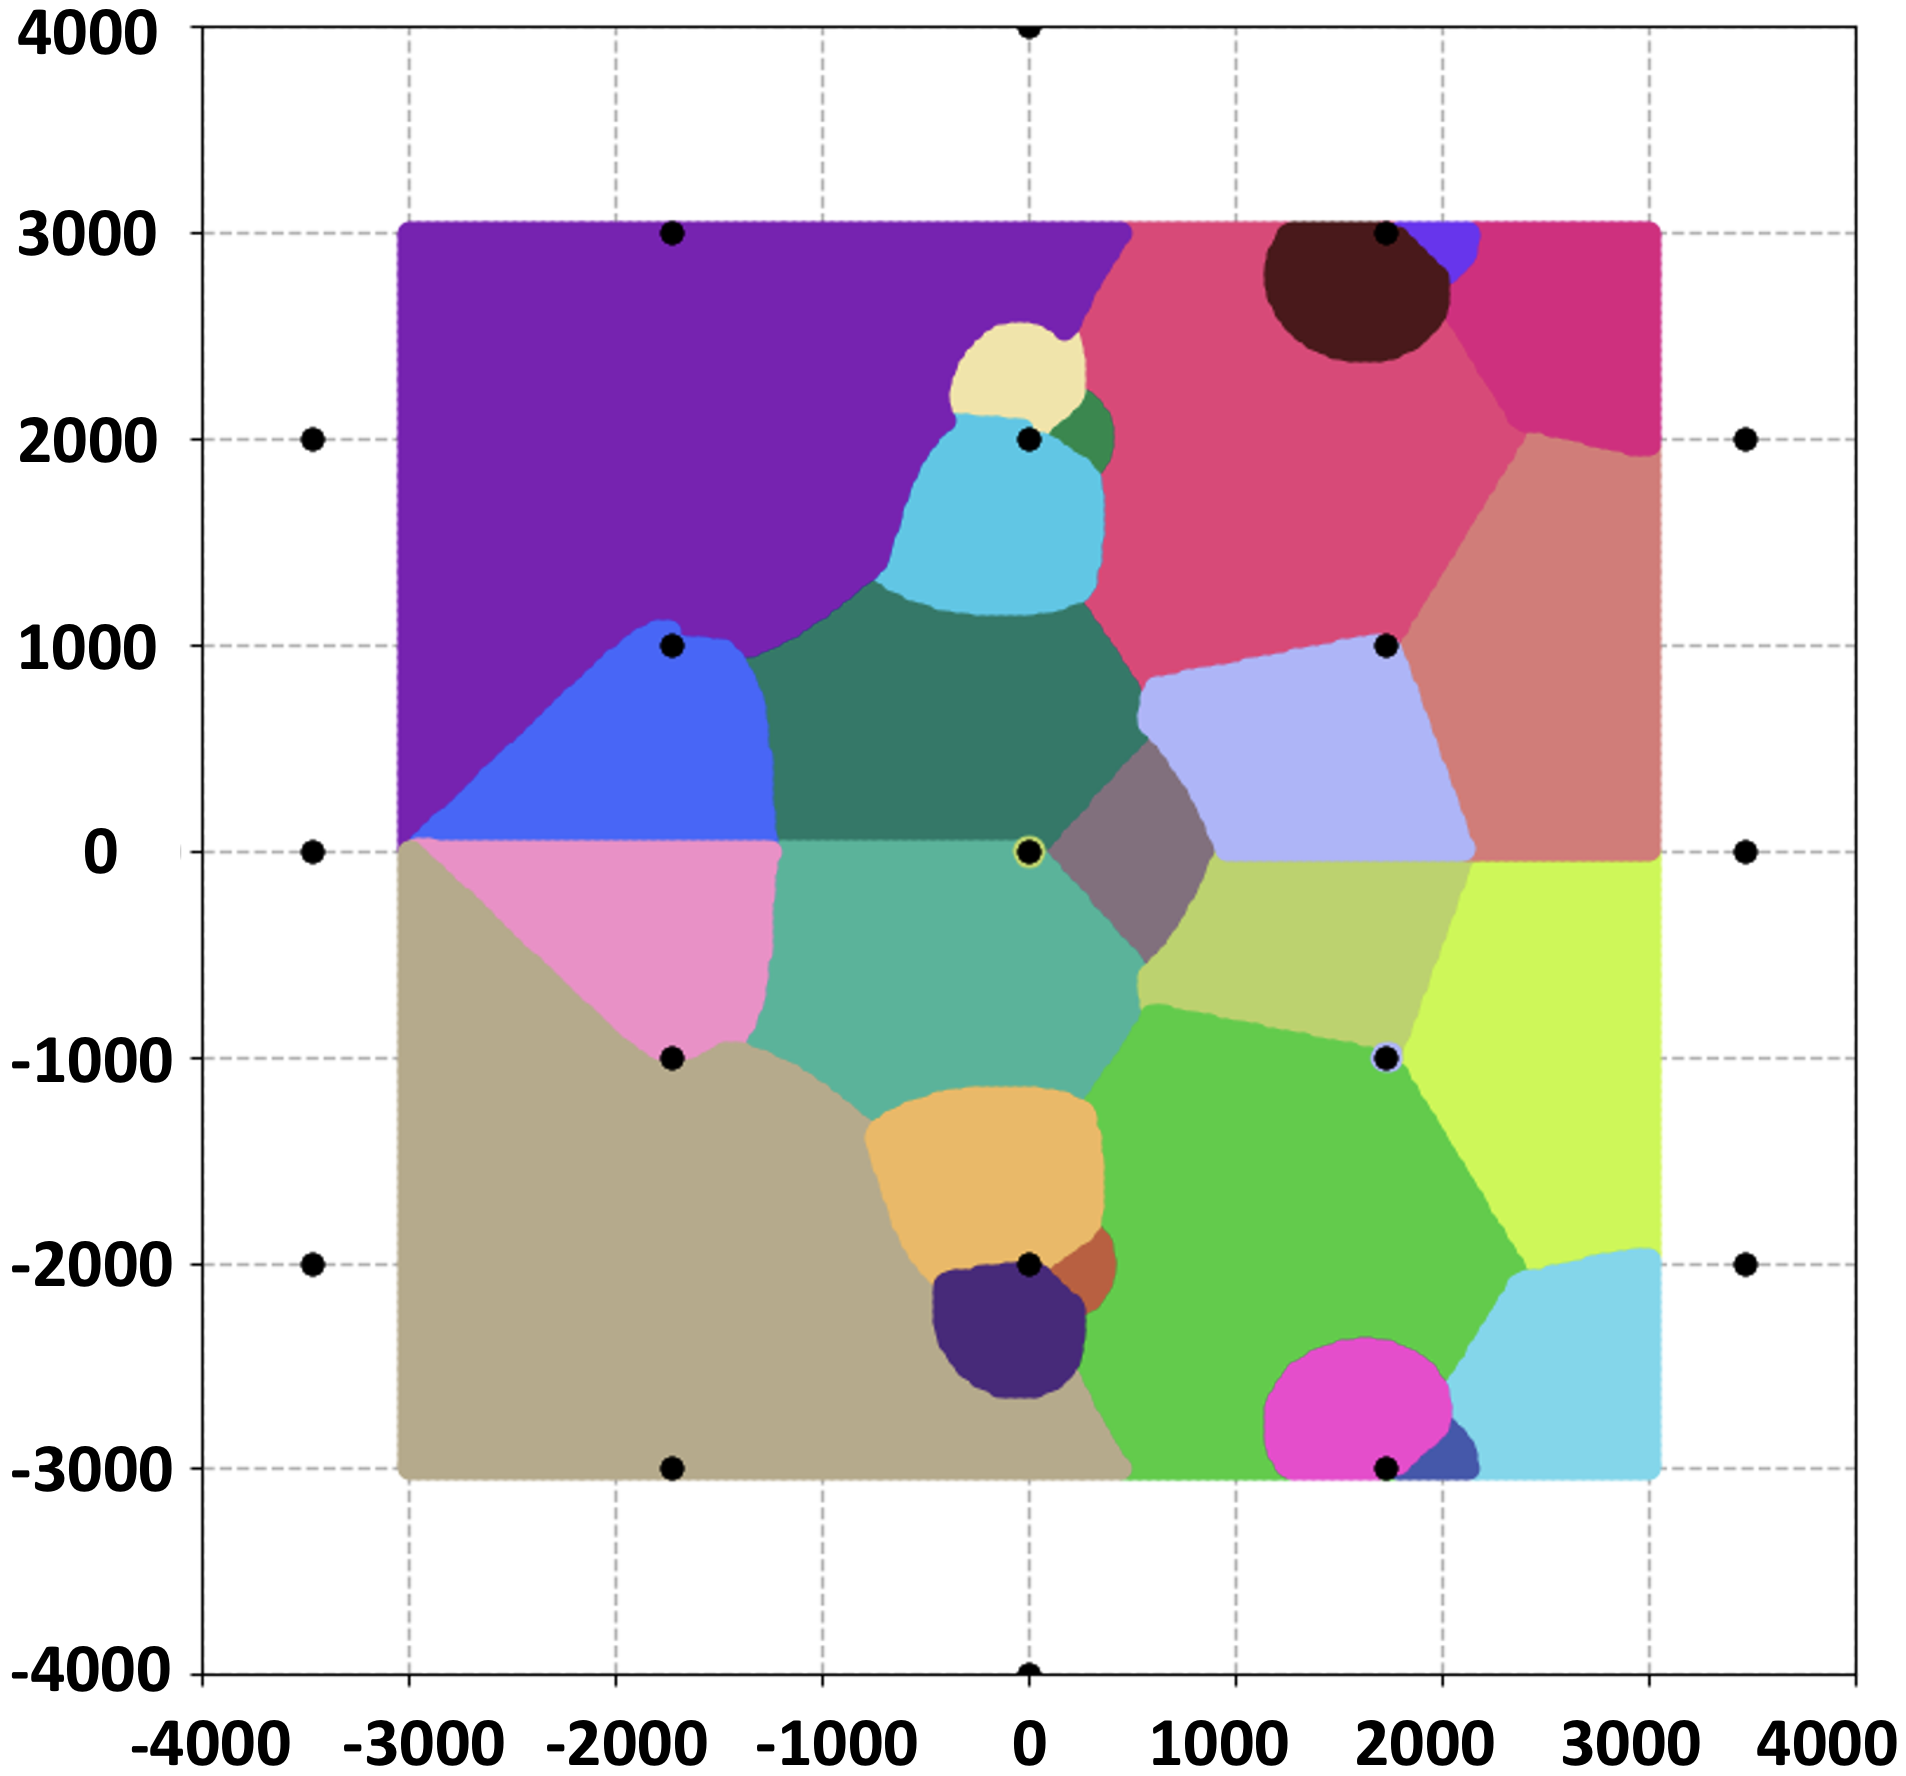
\includegraphics[width=42mm]{Figures/Exemplary-Cell-Partitioning/TWC-SINR-GUE-Very-Large-Cells_2.png}
\label{TWC-Very-Large-Size-GUE}}
\hspace{0mm}
\subfloat[Setup as per Sec.~\ref{experimental-setup} $\times$4.]{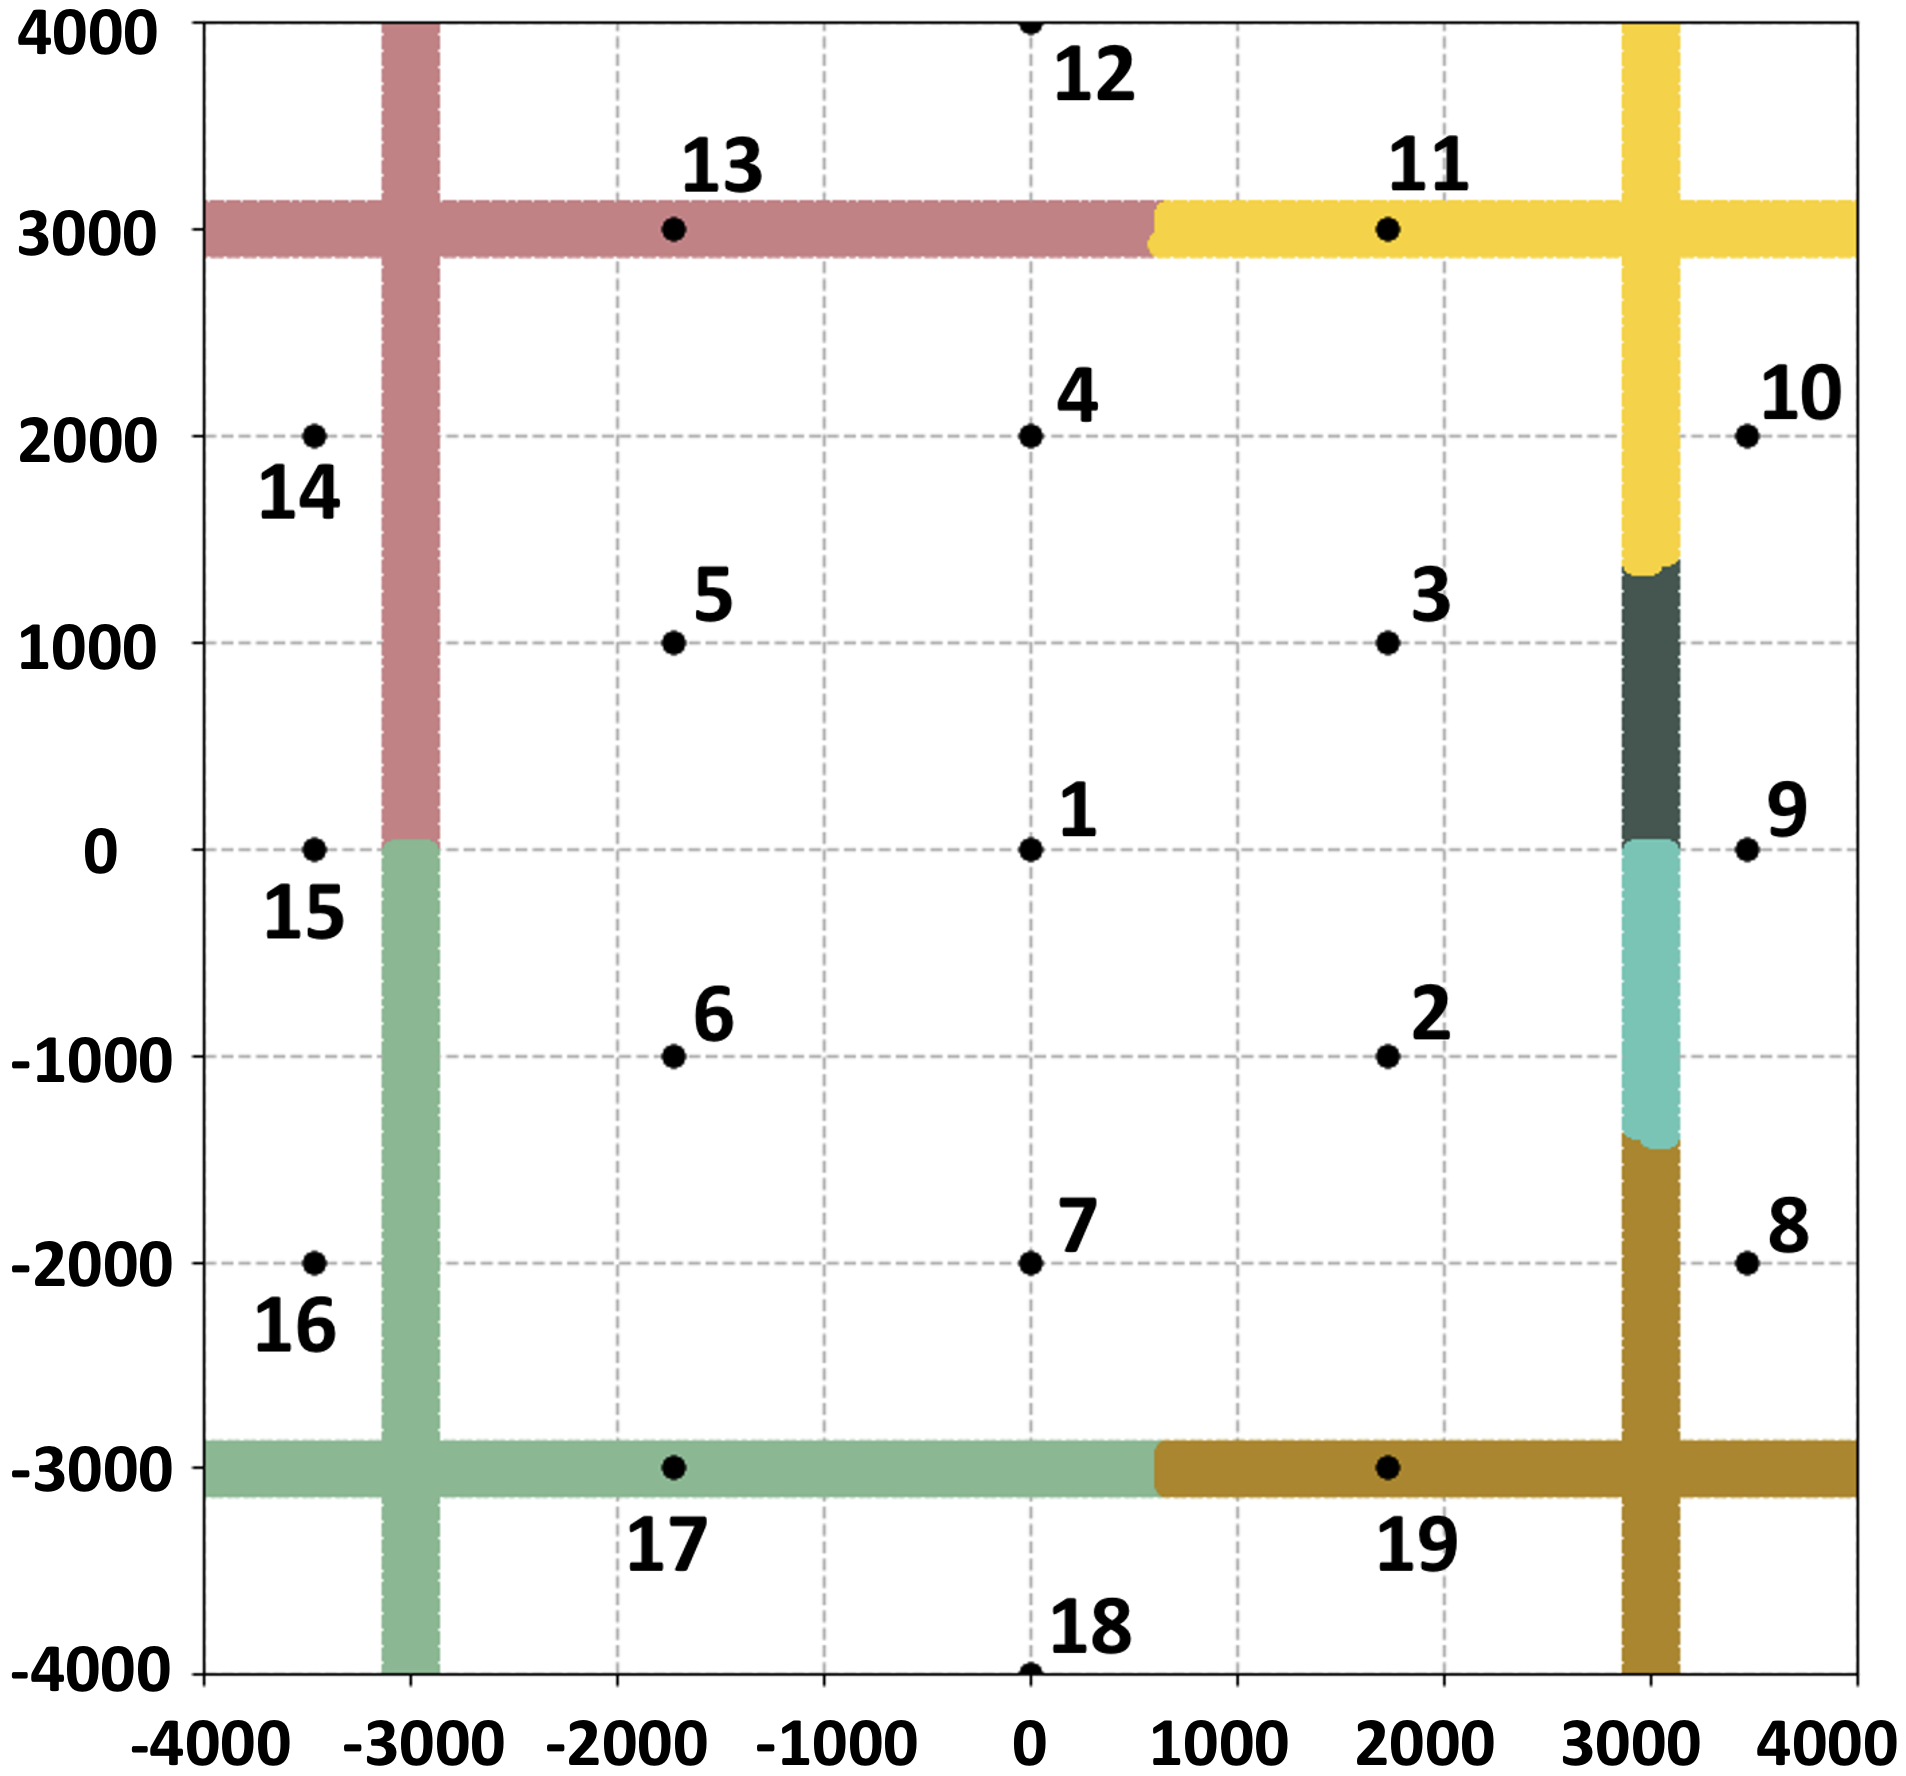
\includegraphics[width=42mm]{Figures/Exemplary-Cell-Partitioning/TWC-very-large-size-UAV-target-region-2.png}
\label{TWC-Very-Large-Size-UAV}}
\hspace{0mm}
\captionsetup{justification=justified}
\caption{Optimized GUEs and UAVs cell partitioning for the Max-SINR-PA-VAT algorithm with $r = 0.5$. Simulations are carried out for three different target region sizes and ISDs.}
%values: \red{(1) Figs. \ref{TWC-Normal-Size-GUE} and \ref{TWC-Normal-Size-UAV} (2) Figs. \ref{TWC-Large-Size-GUE} and \ref{TWC-Large-Size-UAV} (3) Figs. \ref{TWC-Very-Large-Size-GUE} and \ref{TWC-Very-Large-Size-UAV}.}}
\label{TWC-Cell-Partitionings}
\end{figure}
\end{comment}







%%%%%%%%%%%%%%%%%%%%%%%%%%%%%%%%%%%%%%%%

\subsection{Generalization to Probabilistic Line-of-Sight Conditions}\label{Probabilistic-LOS-NLOS}

While the channel setup used for simulations in Section \ref{Experimental-Results} assumed all GUEs to experience a non-line-of-sight (NLoS) condition, our framework is applicable to any given LoS and NLoS set up. Indeed, as per 3GPP channel modeling, the presence or absence of LoS conditions between a user at $\bm{q}$ and its corresponding BS only impacts the specific values of $a_{\bm{q}}$ and $b_{\bm{q}}$ for that particular user. Our framework is designed to accommodate generic values for these parameters. 
For instance, following the 3GPP model \cite{3GPP38901}, if the user location $\bm{q}$ is in the LoS of its corresponding BS, we can take that into account by changing the values of $38.42$\,dB and $30$ in Eqs. (\ref{a_q_values}) and (\ref{b_q_values}) to $34.02$\,dB and $22$, respectively.
%For instance, rather than adopting the values of $38.42$\,dB and $30$ for $a_{\bm{q}}$ and $b_{\bm{q}}$, respectively, when $\bm{q} \in Q_G$ as indicated in Eqs. (\ref{a_q_values}) and (\ref{b_q_values}), these parameters may assume different values, such as $34.02$\,dB and $22$, respectively, if the user location $\bm{q}$ is in a LoS condition w.r.t. its corresponding base station \cite{3GPP38901}. 

Throughout this section, we update the notation from $a_{\bm{q}}$ and $b_{\bm{q}}$ to $a_{\bm{q}, n}$ and $b_{\bm{q}, n}$, respectively, to accommodate the presence or absence of LoS conditions between the user at $\bm{q}$ and BS $n$. In the remainder of this section, we assume that UAVs are consistently in a LoS condition because of their elevated altitude \cite{3GPP36777}; however, the same reasoning can also be applied to user locations $\bm{q} \in Q_U$. Let $\tau_{\bm{q}, n}$ be a binary label taking the value of $1$ if the user location $\bm{q}$ is in LoS with BS $n$ and $0$ otherwise. Then, we have: 
\begin{align}\label{a_qn_values}
a_{\bm{q},n} &=
\begin{cases}
34.02\,\textrm{dB}, & \text{if}\ \bm{q}\in Q_U, \\
34.02\,\textrm{dB}, & \text{if}\ \bm{q}\in Q_G \text{ and } \tau_{\bm{q},n} = 1, \\
38.42\,\textrm{dB}, & \text{if}\ \bm{q}\in Q_G \text{ and } \tau_{\bm{q},n} = 0,
\end{cases}
\\
% \end{equation}
% \begin{equation}\label{b_qn_values}
b_{\bm{q},n} &=
\begin{cases}
22, & \text{if}\ \bm{q}\in Q_U, \\
22, & \text{if}\ \bm{q}\in Q_G \text{ and } \tau_{\bm{q},n} = 1, \\
30, & \text{if}\ \bm{q}\in Q_G \text{ and } \tau_{\bm{q},n} = 0.
\end{cases}
\end{align}
The pathloss in Eq. (\ref{eqn:Pathloss}) is then given by:
\begin{equation} \label{eqn:NewPathloss}
L_{n,\bm{q}} = a_{\bm{q}, n} + b_{\bm{q}, n} \log_{10}\left[\| \bm{q} - \bm{p}_n \|^2 + (h_{\bm{q}} -h_{n,\mathrm{B}})^2 \right]^{\frac{1}{2}},
\end{equation}
while all other notations remain unaltered and all propositions still hold.  


A practical case study for probabilistic LoS conditions follows from the 3GPP standard guideline in which the probability of LoS between the GUE at $\bm{q} \in Q_G$ and BS $n$ located at $\bm{p}_n$ is given by:
\begin{align}\label{probability-LoS}
    \mathrm{Pr}_{\textrm{LoS}} = 
    \begin{cases}
    &\!\!\!\!\! 1,   \qquad\qquad\qquad\qquad\qquad\quad    \text{if}\ \| \bm{q} - \bm{p}_n \| \leq 18\textrm{m}, \\
    &\!\!\!\!\! \frac{18}{\| \bm{q} - \bm{p}_n \|} + \Big(1 - \frac{18}{\| \bm{q} - \bm{p}_n \|}\Big)e^{-\frac{\| \bm{q} - \bm{p}_n \|}{63}},   \quad\textrm{ } \text{otherwise}.
    \end{cases}
\end{align}
For each $\bm{q} \in Q_G$ and $n \in \{1, \cdots, N\}$, the label $\tau_{\bm{q}, n}$ is then created as follows: a scalar $u$ is sampled at random from the uniform distribution $u \sim \mathcal{U}[0, 1]$. The label $\tau_{\bm{q}, n}$ is set to $1$ if $u\leq \mathrm{Pr}_{\textrm{LoS}}$, and $0$ otherwise. Once labels are created, the Max-SINR-PA-VAT algorithm is executed for three scenarios: $r = 0$, $r = 0.5$, and $r = 1$. Fig. \ref{TWC-SINR-CDF-Plot-Prob-LoS} illustrates the CDF of the SINR experienced by GUEs and UAVs in the three different scenarios. Similar observations as the ones in Section~\ref{Resulting-performance-improvement} can be made from this figure, i.e., for $r = 0.5$, there is a tradeoff between optimizing GUE and UAV performance. This tradeoff results in a substantial overall improvement in the SINR perceived by UAVs without a severe degradation in the GUE SINR. %This finding demonstrates the general applicability of our framework and methodology, making it suitable for various ad-hoc practical applications, regardless of the link conditions between users and BSs, and where the latter could even be supplied to the algorithms from available radio coverage datasets.
This finding showcases the broad versatility of our framework and its ability to deal with varying link conditions between users and BSs. Moreover, the algorithms could potentially extract link conditions from existing radio coverage datasets, making our algorithms well-suited for diverse real-world applications.
